\documentclass[11pt, oneside,titlepage]{article}   	% use "amsart" instead of "article" for AMSLaTeX format
\usepackage[margin=1in]{geometry}                		% See geometry.pdf to learn the layout options. There are lots.
\geometry{letterpaper}                   		% ... or a4paper or a5paper or ... 
%\geometry{landscape}                		% Activate for rotated page geometry
\usepackage[parfill]{parskip}    		% Activate to begin paragraphs with an empty line rather than an indent
\usepackage{graphicx}				% Use pdf, png, jpg, or eps§ with pdflatex; use eps in DVI mode
								% TeX will automatically convert eps --> pdf in pdflatex		
\usepackage{amssymb}
\usepackage{etoolbox}
\usepackage{lipsum}
\usepackage{caption}
\usepackage{subcaption}
\usepackage{float}
\usepackage[all]{nowidow}
\usepackage[hang,flushmargin]{footmisc}
\usepackage{slantsc}

    \AfterEndEnvironment{hangparas}{\addvspace{0.67\baselineskip}}
    \usepackage[notquote]{hanging}


\title{\textbf{What (and Whom) to Avoid On the Roads \\ 
\large Analysis of Major Traffic Fatality Predictors}}
\author{Desmond Cole \\
(Time Trends, Automaker/Vehicle Type, Environmental Factors, \\
Report Introduction, General Editing, Conclusion) \\
\\
Teerth Patel \\
(Geographic Trends, Driver Impairment,
General Editing, Conclusion) \\
\\
Yunbin Peng \\
(Hit-and-Run)}

\begin{document}
\interfootnotelinepenalty=10000
\widowpenalty10000
\clubpenalty10000
\maketitle
\section*{Introduction}
\subsection*{Executive Summary}
In the United States, approximately 35-40,000 people die in vehicle-related incidents every year. The fatality rate declined significantly in the second half of the 20th century, and continued to decline in the 21st. However, the decline has plateaued in recent years, to a rate of just over 1 death per 100 million vehicle miles traveled (VMT). Understanding and tackling the problem of crash fatalities has motivated considerable improvements and investments in vehicle design, road design, and scientific knowledge of human motor skills and reaction times. \\ 

With this analysis, we set out to survey the distribution of vehicle-related fatalities across geography and time, and explore a number of driver-specific characteristics to assess dominant contributors to the incidence and extent of vehicle-related deaths. We use this analysis to develop a limited profile of the circumstances associated with traffic fatalities, and a set of corresponding recommendations for the concerned motorist or non-motorist. Our results suggest that luxury autos, daytime driving, and rural areas tend to be the safest circumstances for driving, and that drivers who are impaired (via drugs/alcohol or some mental/physical ailment) are to be avoided.  

\subsection*{Data}
The data used for this analysis are gathered by the National Highway Traffic Safety Administration (NHTSA), a branch of the U.S. Department of Transportation. NHTSA gathers traffic fatality data using the Fatality Analysis Reporting System (FARS), a nationwide census of various information regarding fatalities occurring in motor vehicle crashes. FARS contains a rich set of different features, with information on crash circumstances, areas of damage, police reports, emergency response times, and vehicle characteristics. We focus specifically on data from 2015 and 2016, and subset a choice set of predictors of interest, paying particular attention to the following broad indicators of driver behavior:

\begin{enumerate}
\item Where do they drive?
\begin{itemize}
\item Key Variable: Geographic Location
\end{itemize}
\item When do they drive?
\begin{itemize}
\item Key Variable: Time of Day
\end{itemize}
\item What do they drive?
\begin{itemize}
\item Key Variables: Automaker, Vehicle Type
\end{itemize}
\item Are they impaired?
\begin{itemize}
\item Key Variable: Drug/Alcohol Consumption
\end{itemize}
\item Do they flee collisions?
\begin{itemize}
\item Key Variable: Hit-and-Run
\end{itemize}
\end{enumerate}

\section*{Exploratory Analysis and Visualization}

We begin with a geographic and time-based overview of patterns of fatal traffic incidents.

\subsection*{Geographic Patterns}

We begin with a geographical overview of where most fatal accidents occur, shown in the below plot of the United States. Plotting where fatal accidents occur provides both a measure of areas of high geographic risk and suggests certain variables to consider/evaluate (for example, urbanicity).

\begin{figure}[H]
\centering
  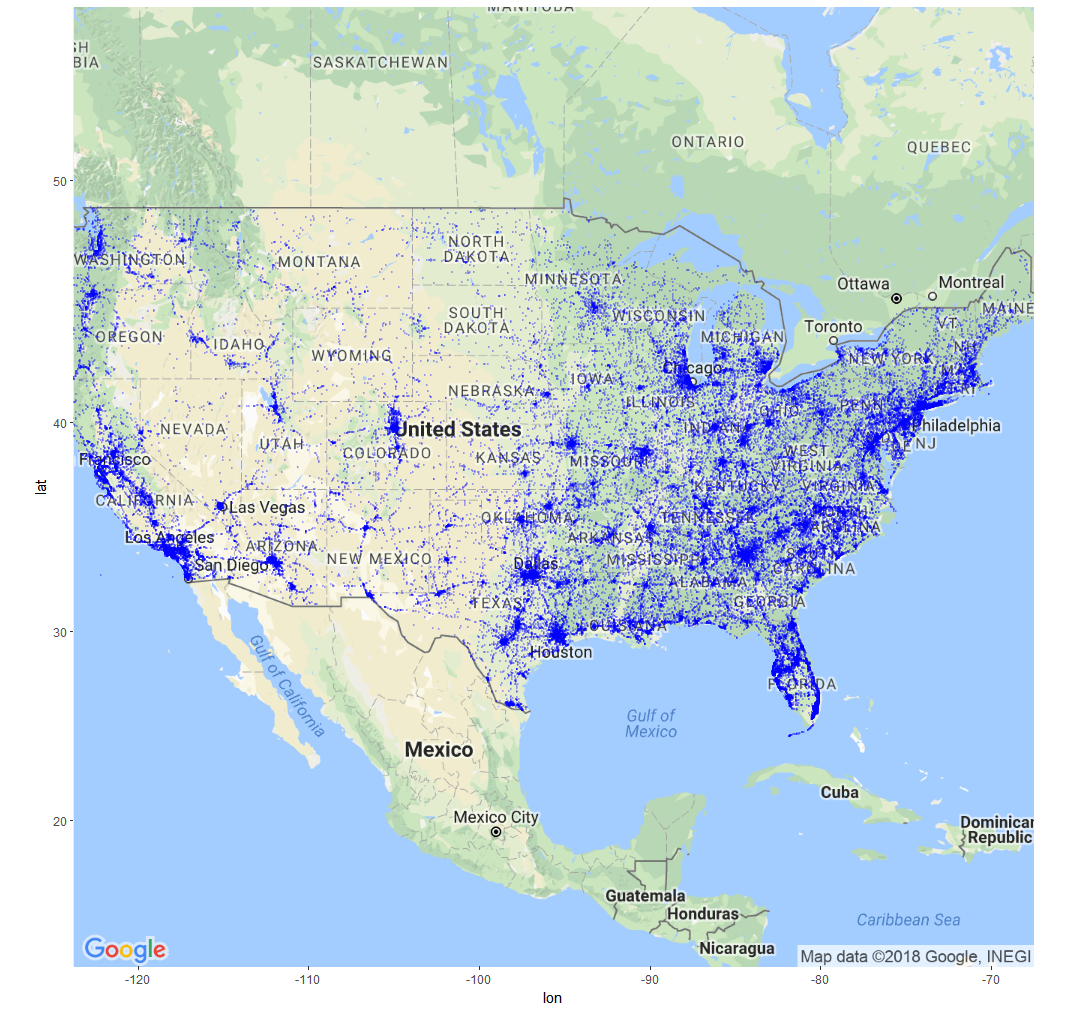
\includegraphics[width=15cm,height=10cm,keepaspectratio]{heatmap.png}
\caption{Heatmap of all fatal accidents}
\end{figure}

Figure 1 shows that the majority of fatal accidents happen on the East Coast, around major cities and areas that are much more populous. This weighs against the notion that that high speed may not be as large a factor of fatal accidents as expected, as areas of low population would be expected of having a higher rate of speeding. The notion that high populous areas have more fatal accidents is fairly trivial. However, what is not obvious is the fact that the accidents actually occur on the major roads and highways much more often. Most of the fatal accidents can be seen to occur on the highways in Figure 1. This suggests that road type is an important factor to consider.

\begin{figure}[H]
\centering
  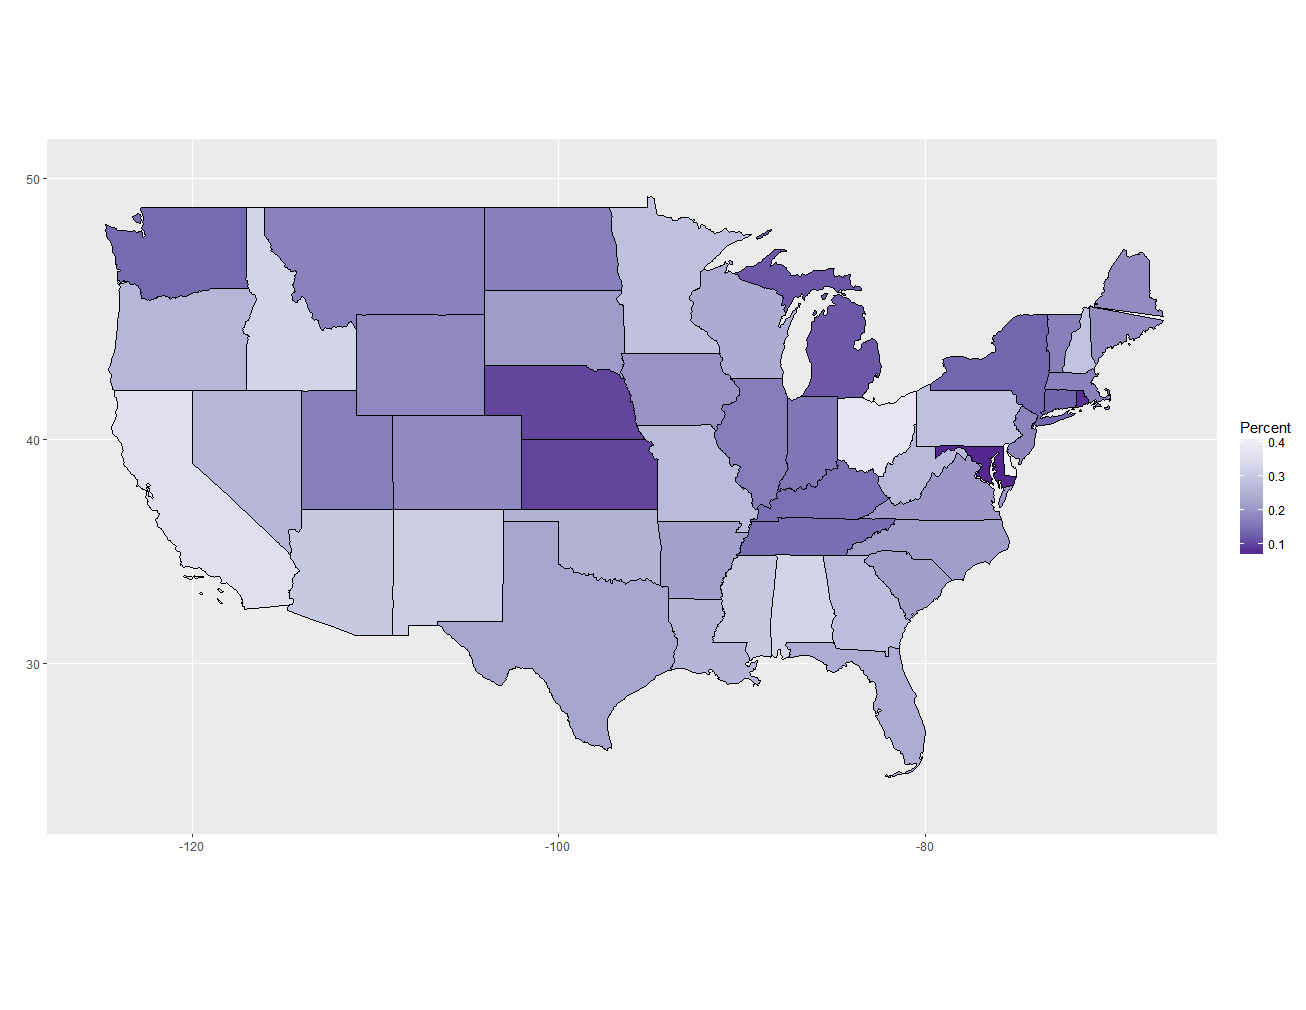
\includegraphics[width=15cm,height=8cm,keepaspectratio]{choropleth.png}
\caption{Choropleth of Accidents per 1000 people per state}
\end{figure}

Observing accidents over population shows a different perspective of where fatal accidents occur. Idaho, for instance, had few incidences of fatal accidents in Figure 1, but when we look at Figure 2, Idaho has one of the highest proportions of accidents. Similarly, we can see that places that have high concentrations of fatal accidents, such as New York, Michigan, Kentucky, and Maryland, actually have much lower proportion of accidents per capita. Also, the more densely populated areas seem to have the highest number of fatal accidents per capita.

\subsection*{Time Trends - Hourly Cycle}
At the national and state level, the cycle of fatal accidents throughout the day is fairly consistent. The below plot shows aggregate fatal accidents per thousand vehicles per hour for the United States, between 2015 and 2016. To account for traffic variability, we weighted the rate of fatal incidents according to hour-by-hour traffic flow allocations estimated by Batterman, et al. (see references). These same flow allocations are used to weight state-by-state hourly trends, under the assumption that state-by-state traffic flow patterns tend to be similar. \\

At the state level, the daily fatal accident cycle is roughly similar. Estimating the overall traffic flow for each state using state-level vehicle registrations, combined with the flow allocations estimated by Batterman, et al. (2015), returns state-level cycles that closely mirror the overall national trend.

\begin{figure}[H]
\centering
\begin{subfigure}{.5\textwidth}
	\centering
	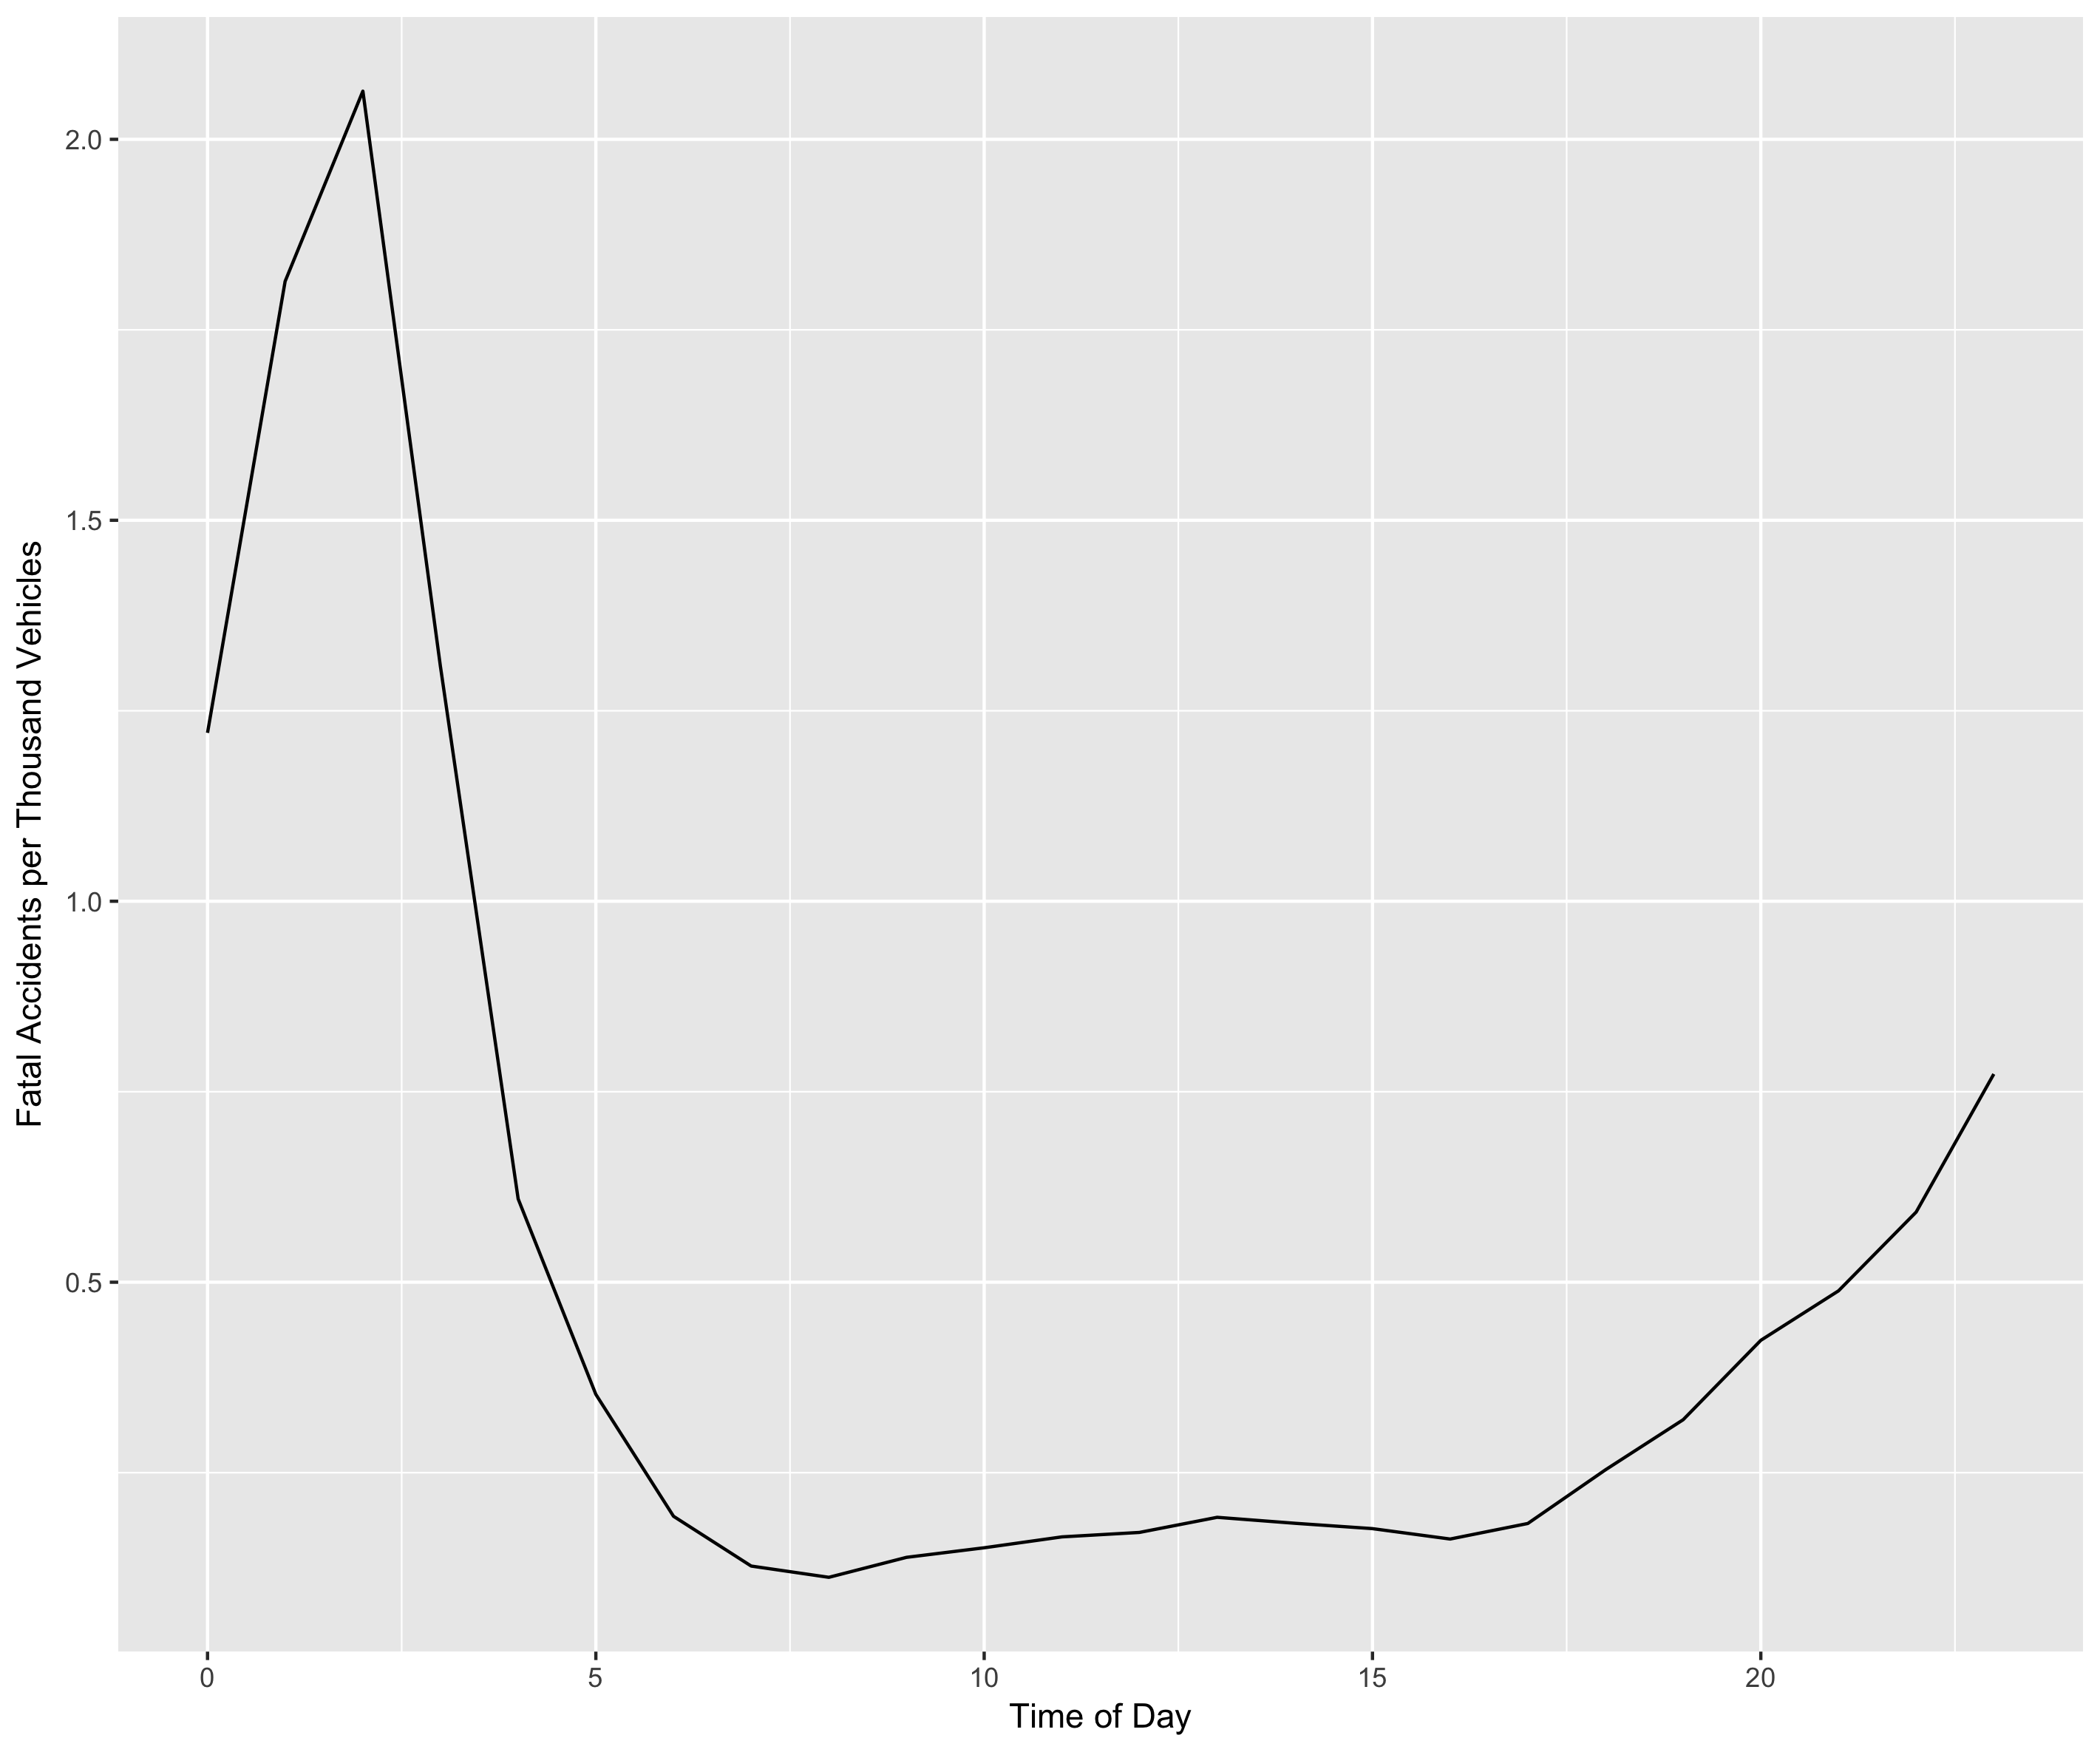
\includegraphics[width=.9\textwidth,height=9cm,keepaspectratio]{WeightedNationalDayTrends.png}
	\caption{National Daily Trend}
	\label{fig:sub1}
\end{subfigure}%
\begin{subfigure}{.5\textwidth}
  \centering
	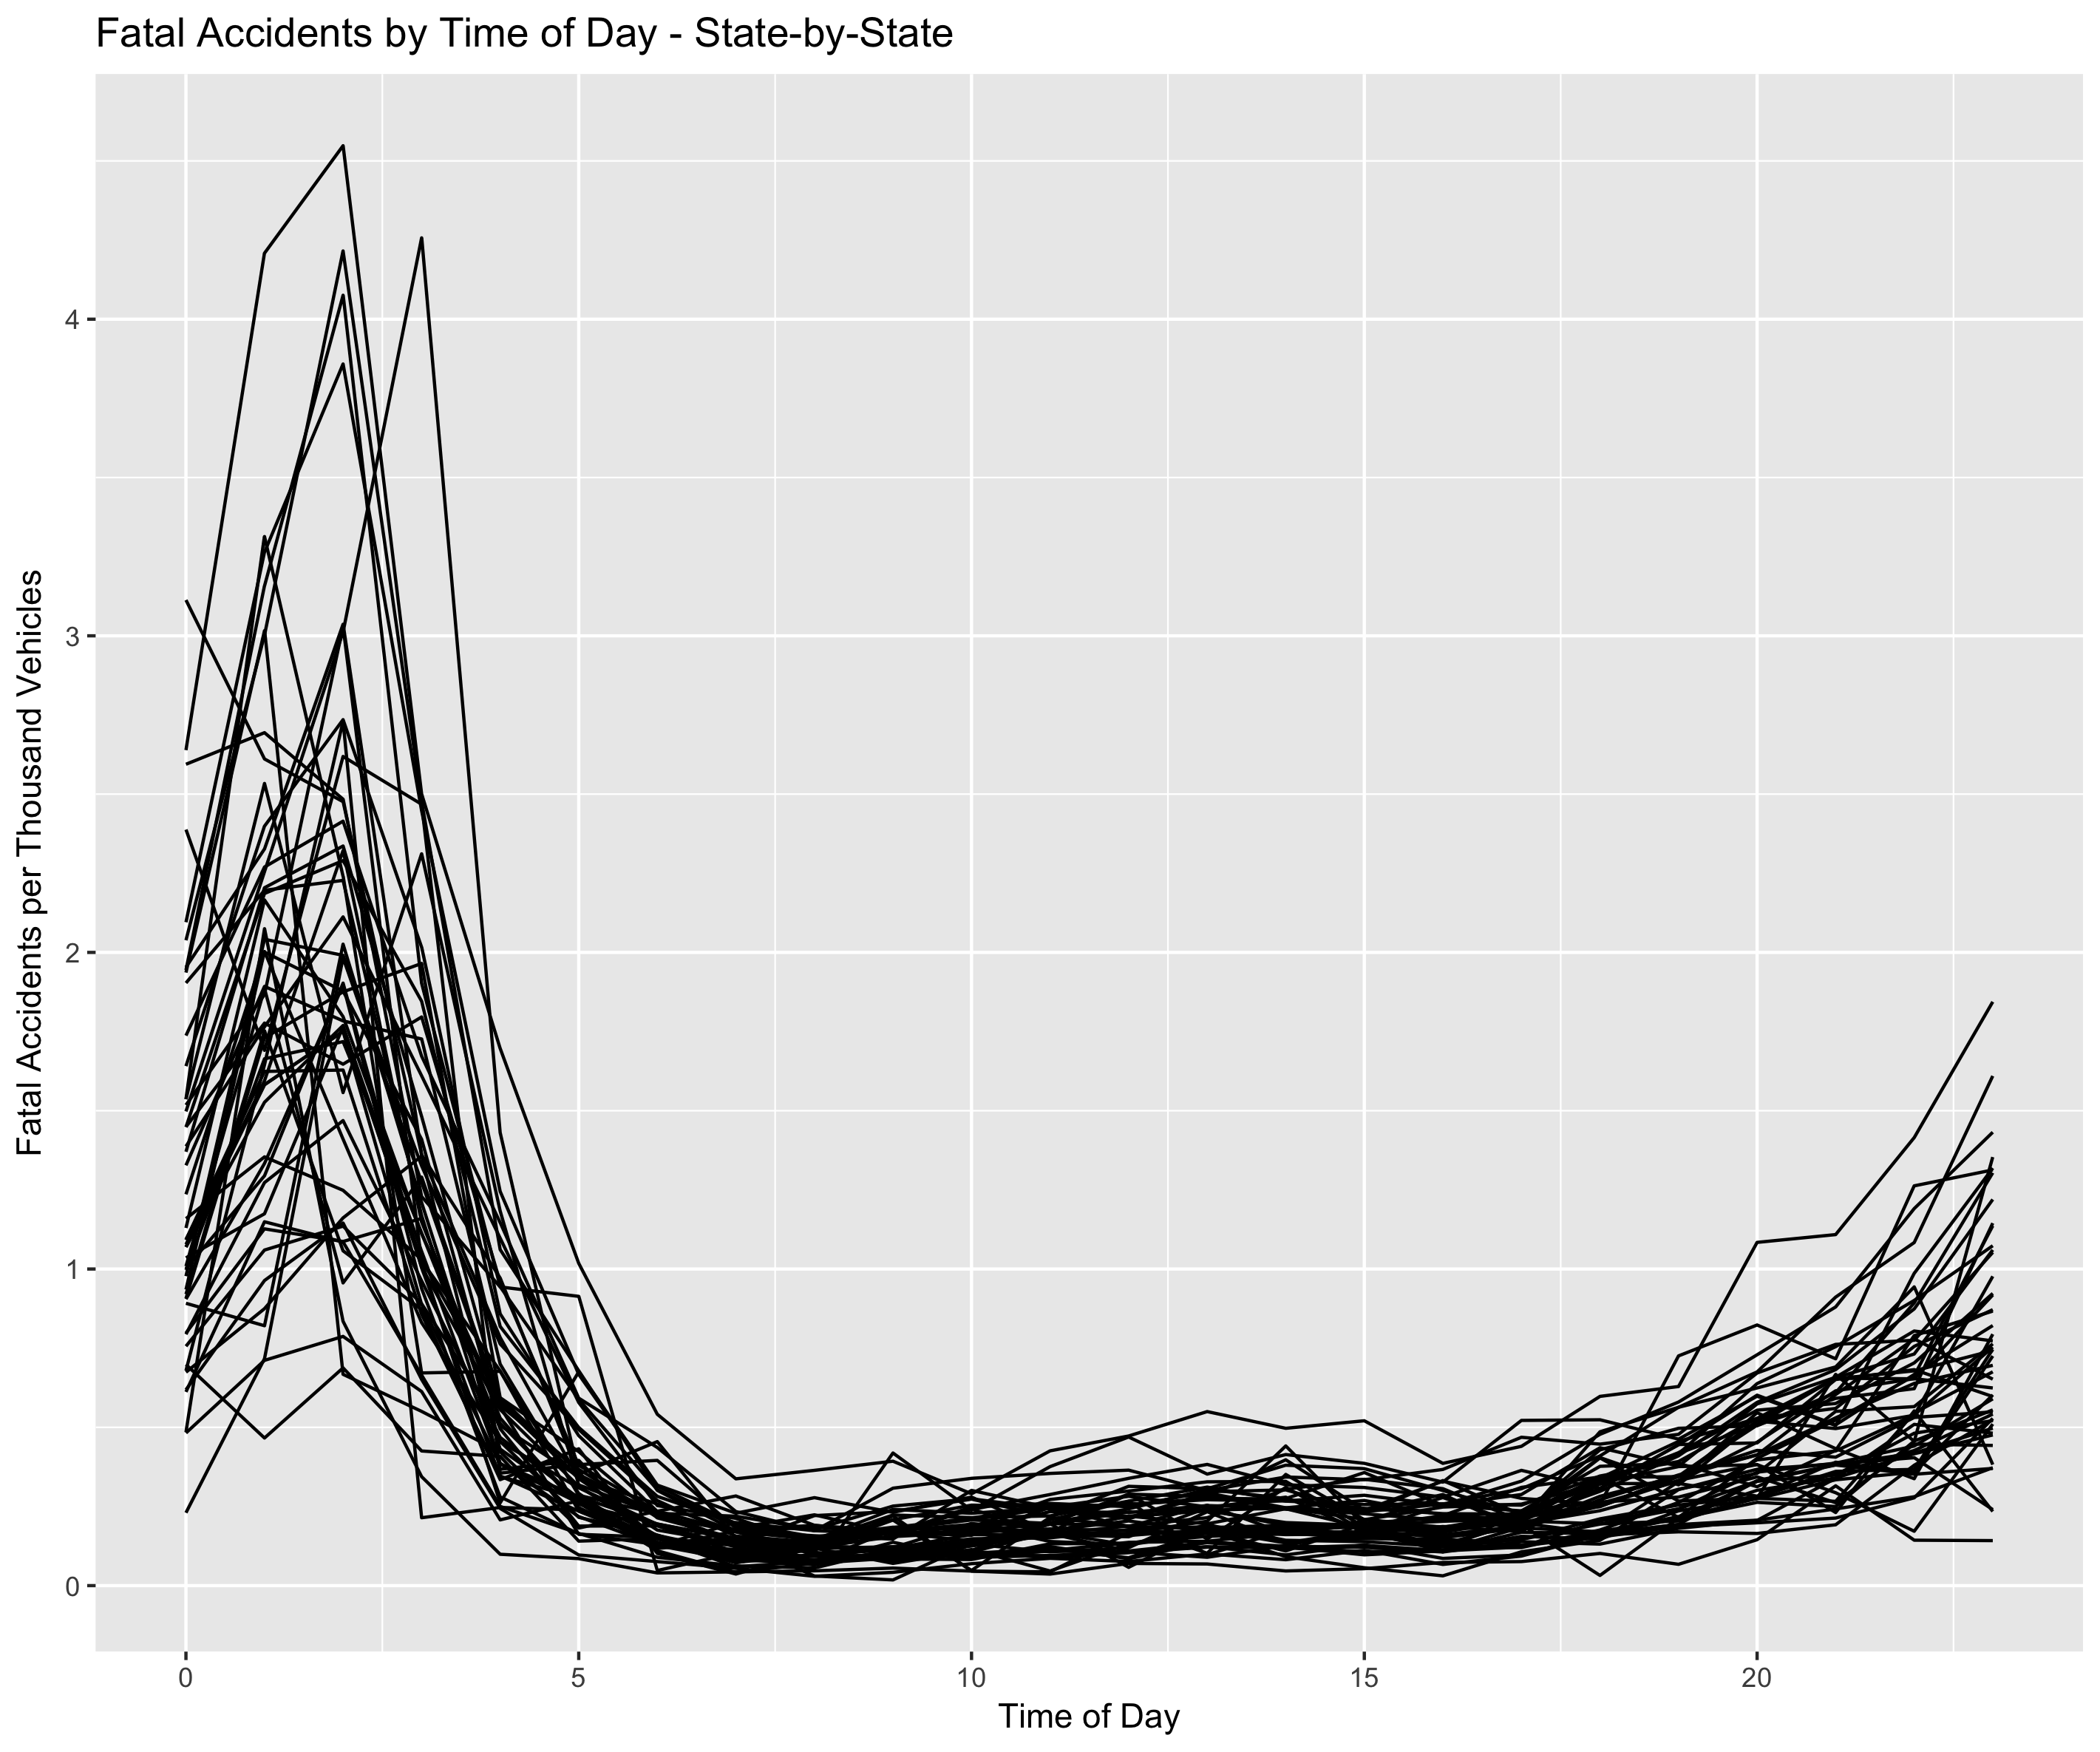
\includegraphics[width=.9\textwidth, height=9cm,keepaspectratio]{WeightedStatePlot.png}
	\caption{State-by-State Daily Trend}
  \label{fig:sub2}
\end{subfigure}
\caption{National and State-by-State Fatal Accident Daily Trends}
\label{fig:test}
\end{figure}

To tease out potential state-level variation in daily cycles, we used shape-based time series clustering, available in R's dtwclust package. Roughly speaking, this method clusters different time series based on their similarity to different centroids, where a centroid in this case is some typical time trend. Further detail on relevant methods is available in work by Gravano and Paparrizos (2015). Testing different numbers of clusters yielded little overall diversity in terms of performance. A plot of results obtained using 2 clusters is below.\footnote{Across multiple iterations, a 2-cluster separation tends to yield the best performance. For reference in the Validity Index table, optimal clustering will minimize the Silhouette (``Sil"), Davies-Bouldin (``DB" and ``DBstar") indices, and maximize the Dunn index (``D"), Calinski-Harabasz index (``CH"), and Score Function (``SF"). 2 clusters were chosen to be optimal on this basis.} There is little indication of significant variation across clusters, and the clustering results (and performance statistics, shown in the below table) are highly sensitive to initial randomization. 

\begin{figure}[H]
\begin{center}
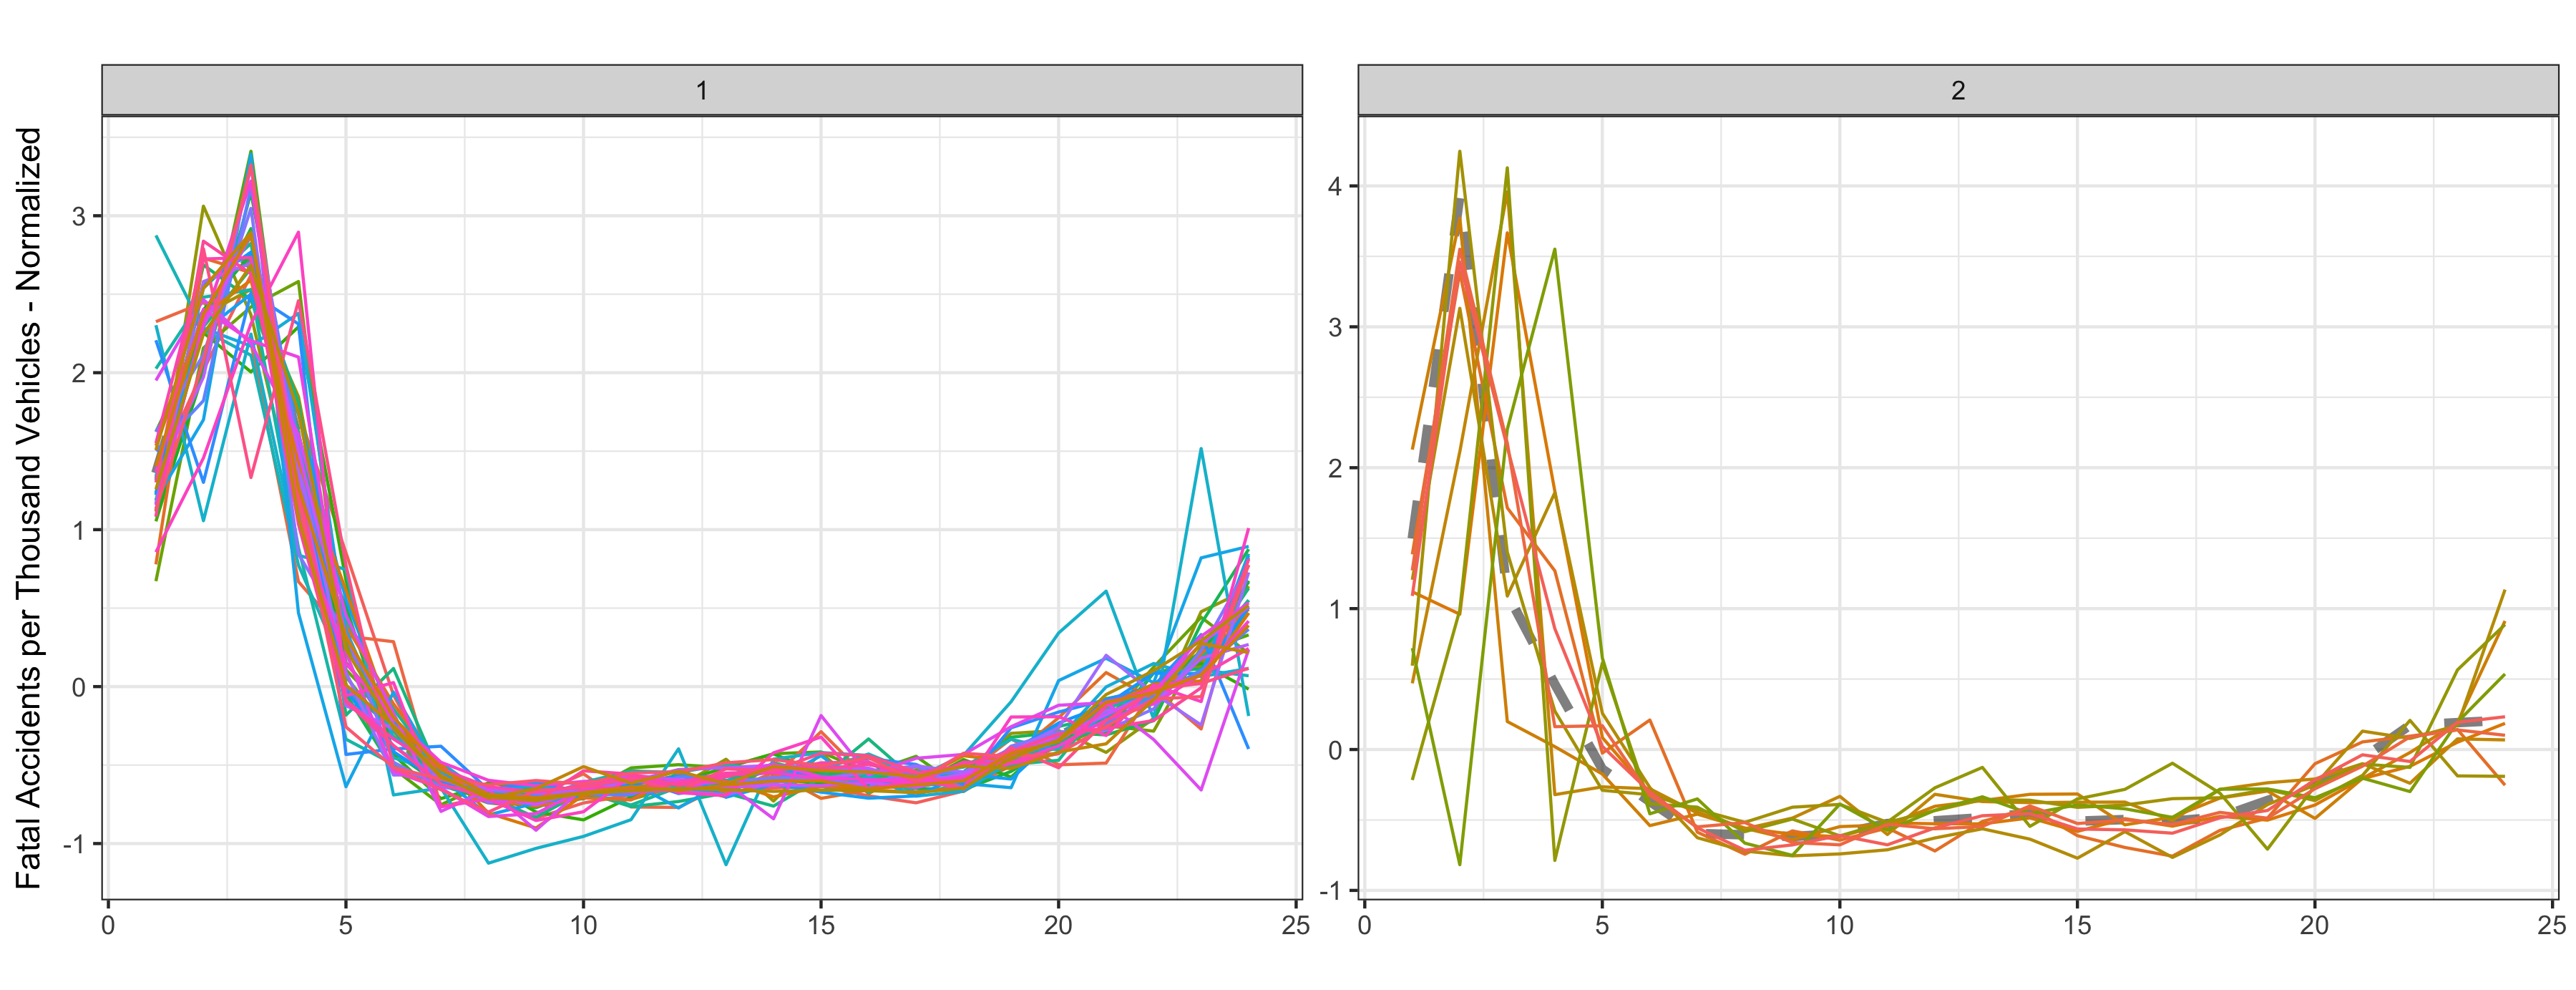
\includegraphics[width=.75\textwidth,height=6cm,keepaspectratio]{StateClusterPlot_Hourly.png}
\end{center}
\caption{Clusters of States By Daily Fatal Accident Trends}
\end{figure}

\begin{table}[H]
\centering
\begin{tabular}{rrrrrrrrr}
  \hline
 NumClusters & Sil & SF & CH & DB & DBstar & D & COP \\ 
  \hline
  2 & 0.508 & 0.602 & 23.664 & 0.899 & 0.899 & 0.072 & 0.181 \\ 
  3 & 0.267 & 0.595 & 17.453 & 1.461 & 2.080 & 0.013 & 0.135 \\ 
  4 & 0.167 & 0.589 & 12.171 & 1.929 & 2.510 & 0.019 & 0.121 \\ 
  5 & 0.133 & 0.572 & 9.163 & 1.345 & 2.451 & 0.017 & 0.153 \\ 
  6 & 0.391 & 0.576 & 15.172 & 0.683 & 1.219 & 0.056 & 0.084 \\ 
   \hline
\end{tabular}
\caption{Time Series Cluster Validity Indices (CVIs)} 
\end{table}


\section*{Traffic Fatality Risk Factor Analysis}
We used a mix of classifiers to assess factors relevant to incident fatalities, with a particular focus on driver behavior and vehicle manufacturer. Our analysis begins with an overview of vehicle types/manufacturers, focusing on their relevance within the context of other predictors. We then separately examine different aspects of driver behavior, specifically driver impairment and whether a driver engaged in a hit-and-run during a given collision. Given that our dataset consists solely of fatal traffic incidents, we choose as a primary output incidents involving more than one fatality.

In several cases, we had to grapple with significant class imbalance. For example, there are far more single-fatality incidents than multi-fatality incidents. As a result, optimal classification in the naive setting without any resampling will occasionally identify all incidents as single-fatality.   

\subsection*{Automakers}

This section explores in some detail different fatality rates for different car types (by automaker, vehicle body, etc.).\footnote{Note that the numbers in this assessment focus on car brands \textit{involved} in fatal incidents. Thus, they do not imply specifically that the vehicle types considered here actually caused death(s), or that the driver(s) of the vehicle(s) themselves died.} For this assessment, we focused on the 15 largest automakers that together produce more than 95\% of the cars and light trucks on American roads. In addition, we subsetted the data to focus specifically on smaller vehicles, excluding commercial vehicles, semi-trucks, etc. \\

The plot below shows a basic ranking of car manufacturers according to the number of fatalities per million vehicles. This is scaled and subsetted according to an approximation of the number and types of vehicles each manufacturer has on the road, but due to a lack of thorough data, it is likely that not all variation simply attributable to manufacturer size and vehicle class has been accounted for. With that said, this plot does suggest that there is meaningful variation across manufacturers in terms of their safety record, with makers such as Subaru and luxury makers such as BMW and Land Rover having significantly less involvement in fatal incidents than carmakers like GM, Ford, and Volvo.
\\
\begin{figure}[H]
\begin{center}
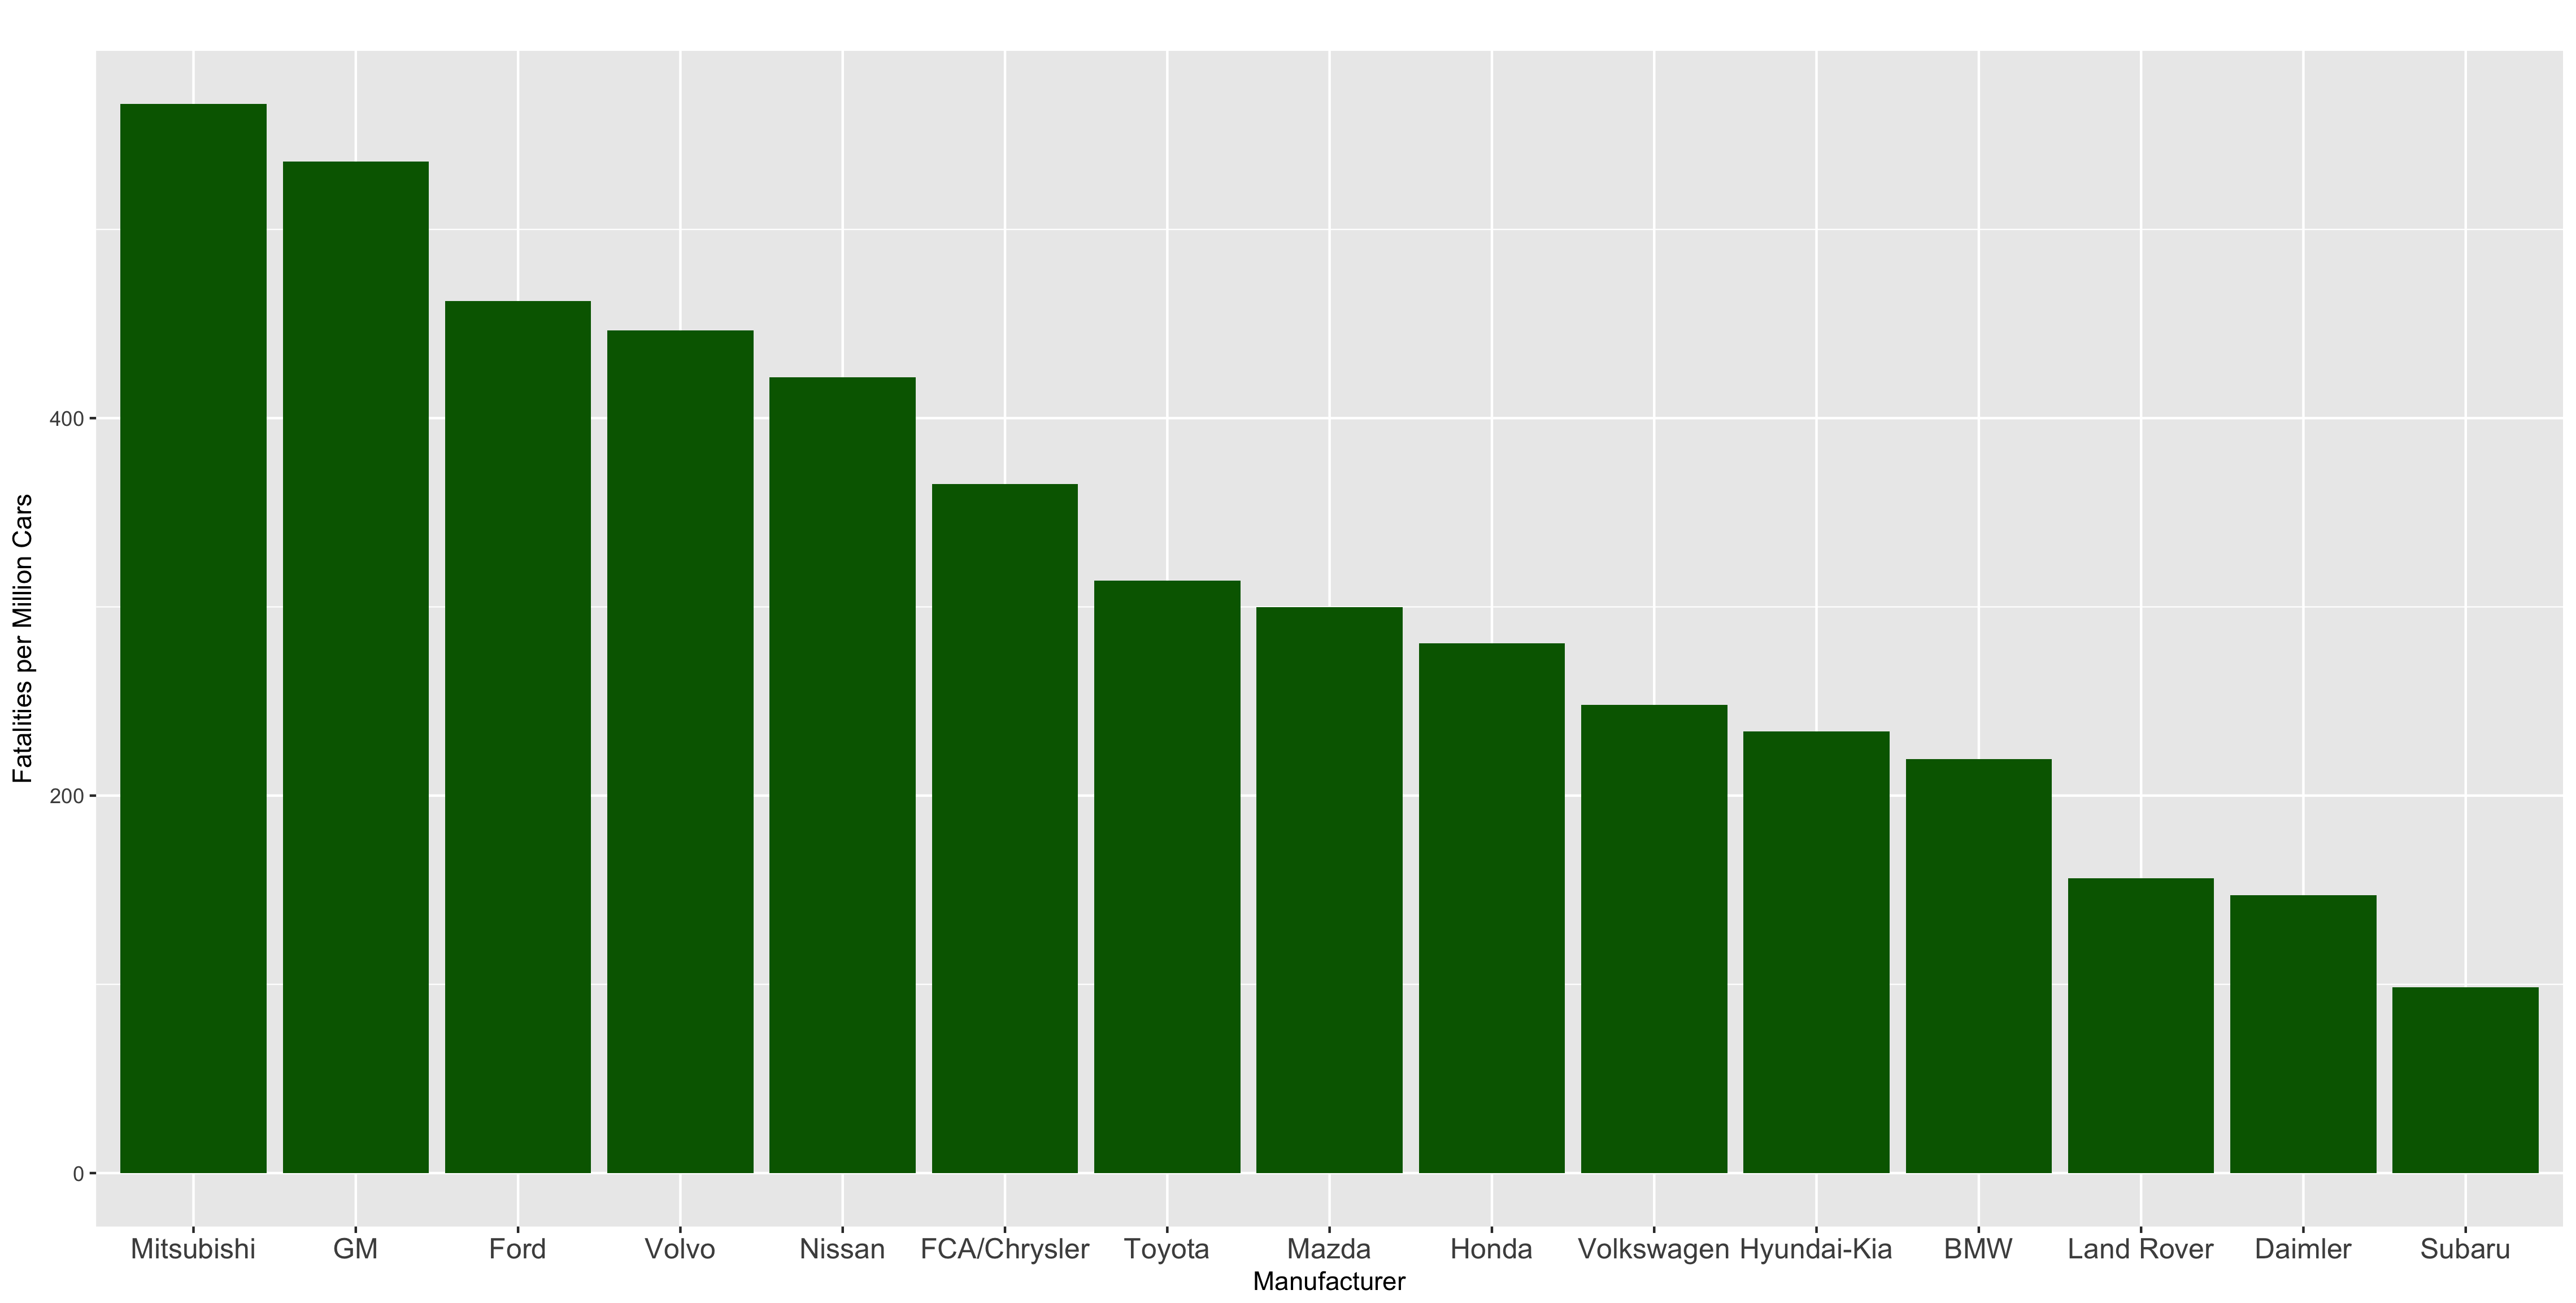
\includegraphics[width=.9\textwidth]{ManufacturerRankingPlot.png}
\end{center}
\caption{Ranking of Manufacturer by Fatal Accidents}
\end{figure}

Although suggestive of meaningful difference across manufacturers, a simple comparison of automakers fails to fully account for the various contextual differences across vehicle types which may be unobservable. To further explore the potential relevance of car manufacturer and car type to crash risks, we applied multidimensional scaling to visually assess the differences between vehicles in terms of various driver-specific crash-relevant pieces of information, such as use of restraints, drug/alcohol use, fires, and speeding, with the goal being to assess whether a certain vehicle type or manufacturer predicts the behavior of the vehicle's driver. To potentially support interpretation of this plot, we included in subfigure (b) a distance-based plot of different vehicle classifications (i.e. Luxury, Non-luxury). \\

\begin{figure}[H]
\centering
\begin{subfigure}{.5\textwidth}
	\centering
	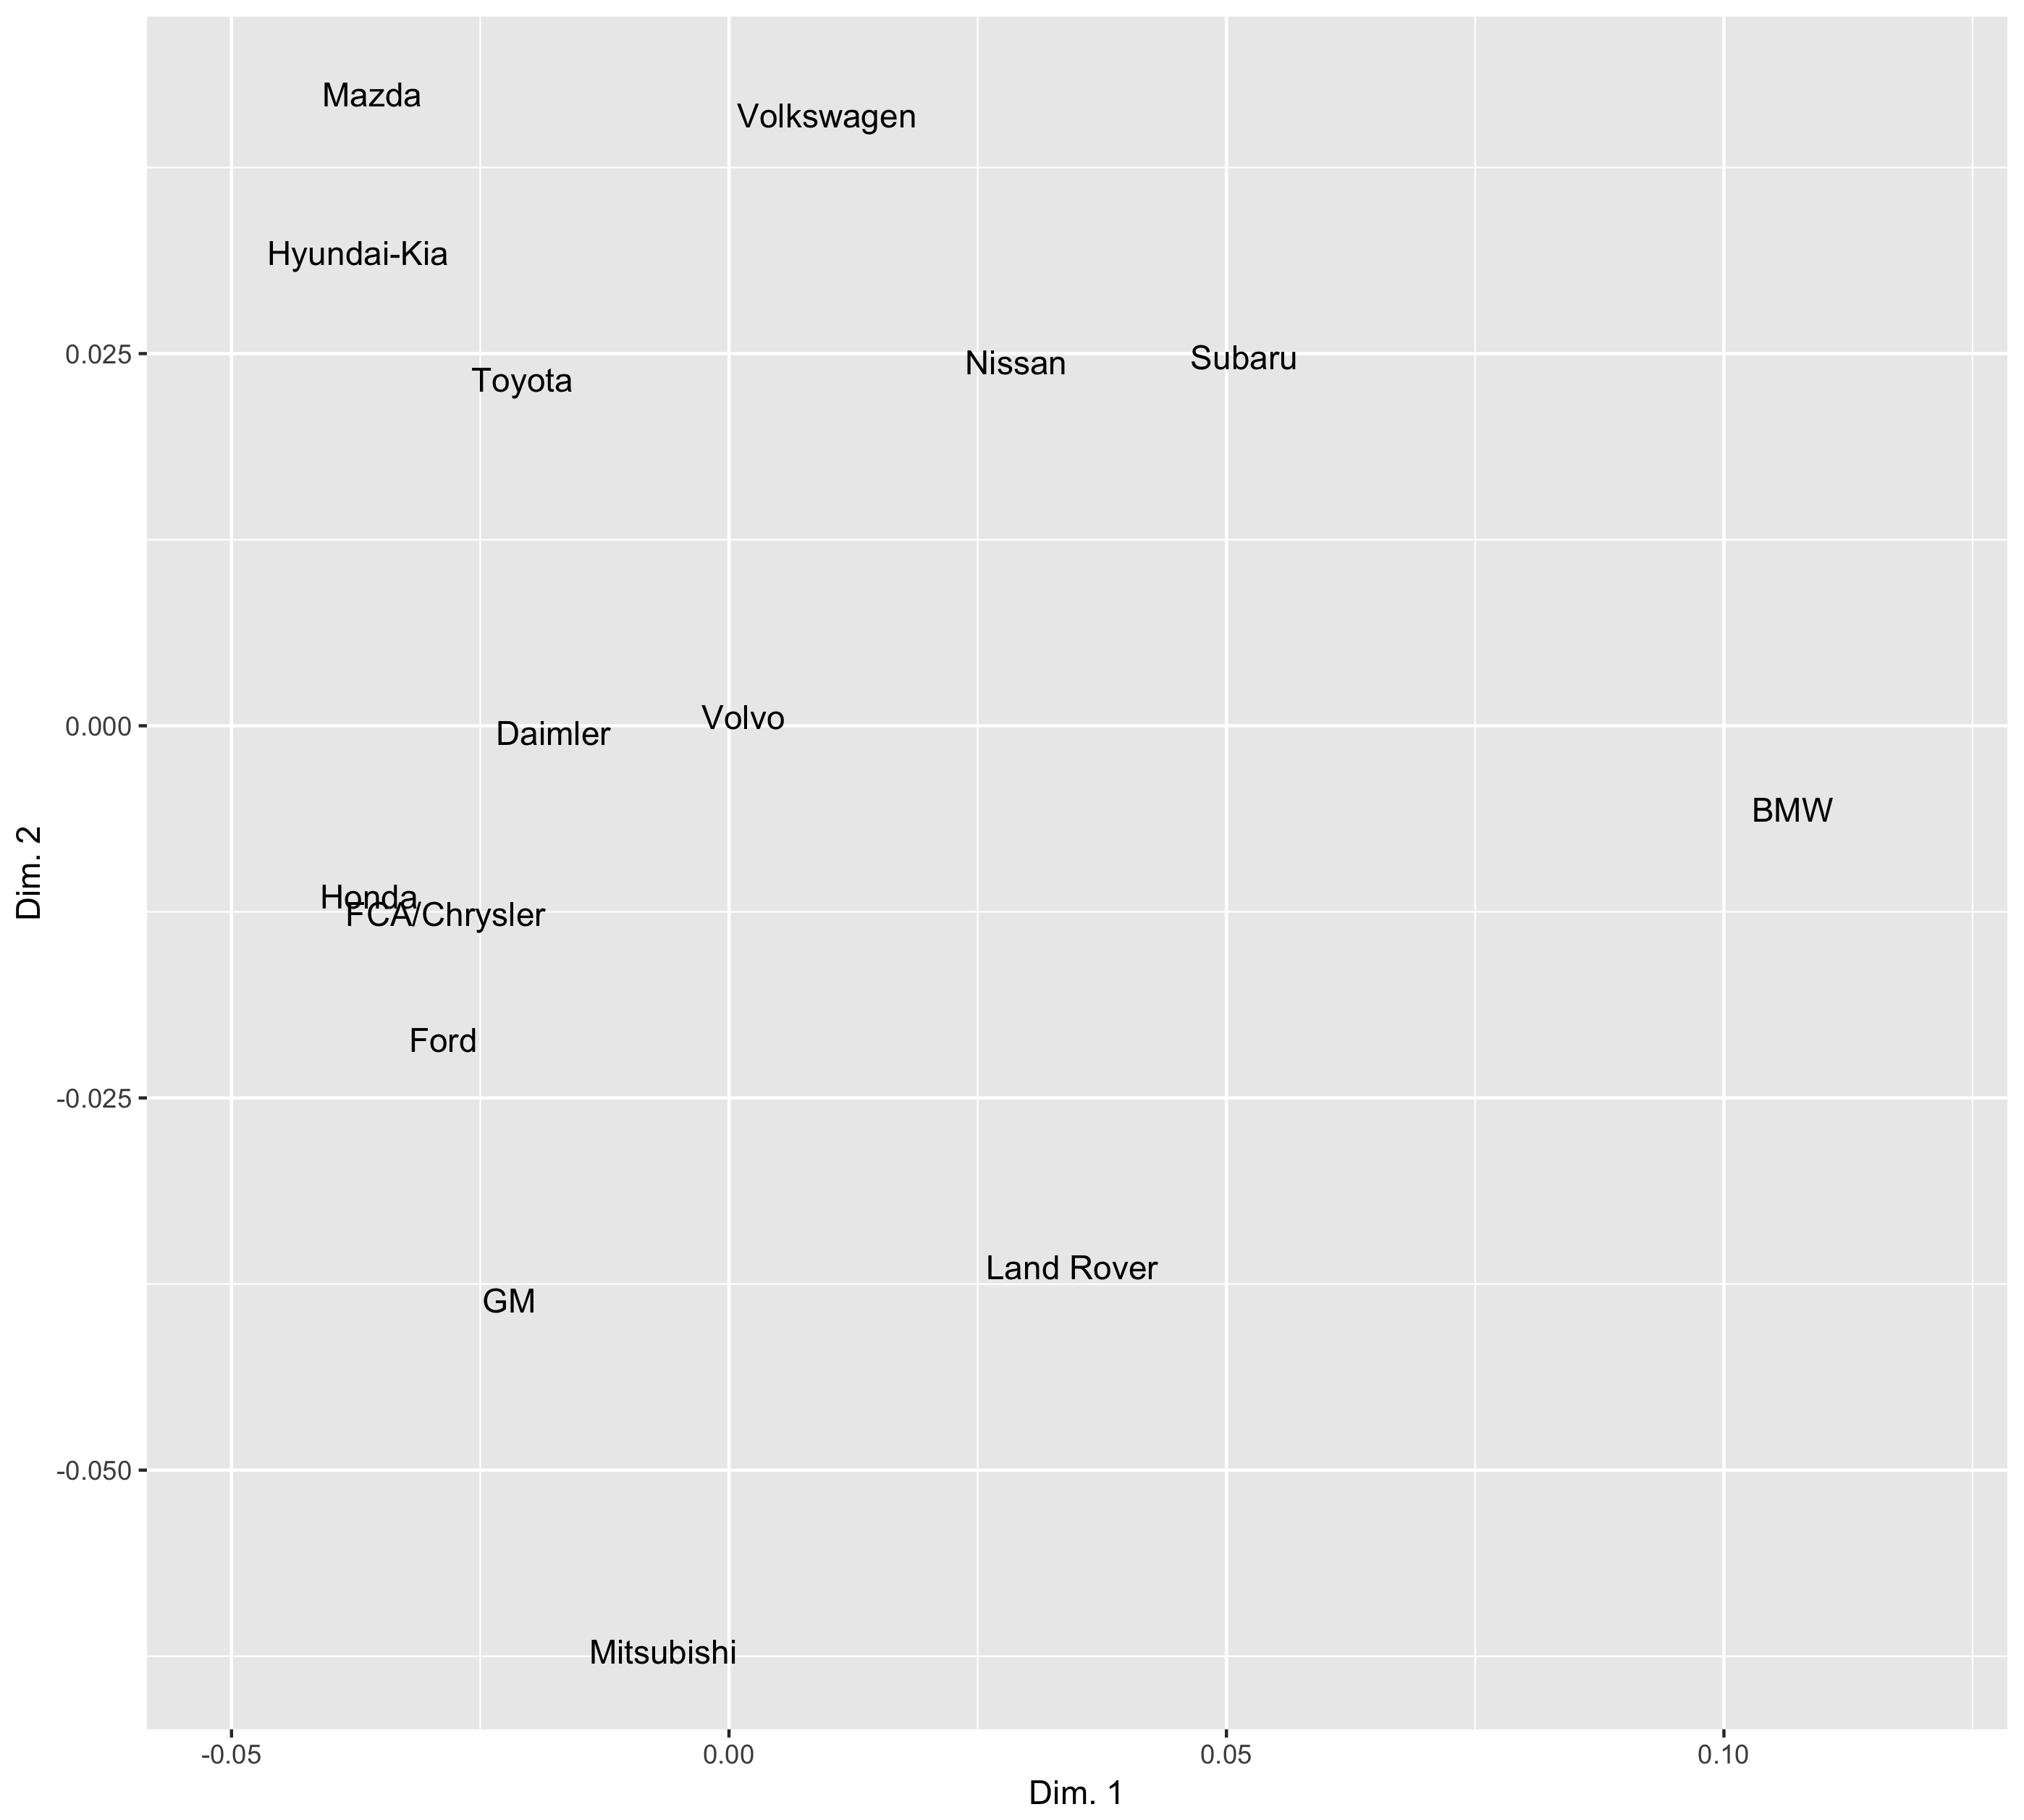
\includegraphics[width=1\linewidth]{ManufacturerMDSPlot.png}
	\caption{Manufacturer MDS}
	\label{fig:sub1}
\end{subfigure}%
\begin{subfigure}{.5\textwidth}
  \centering
  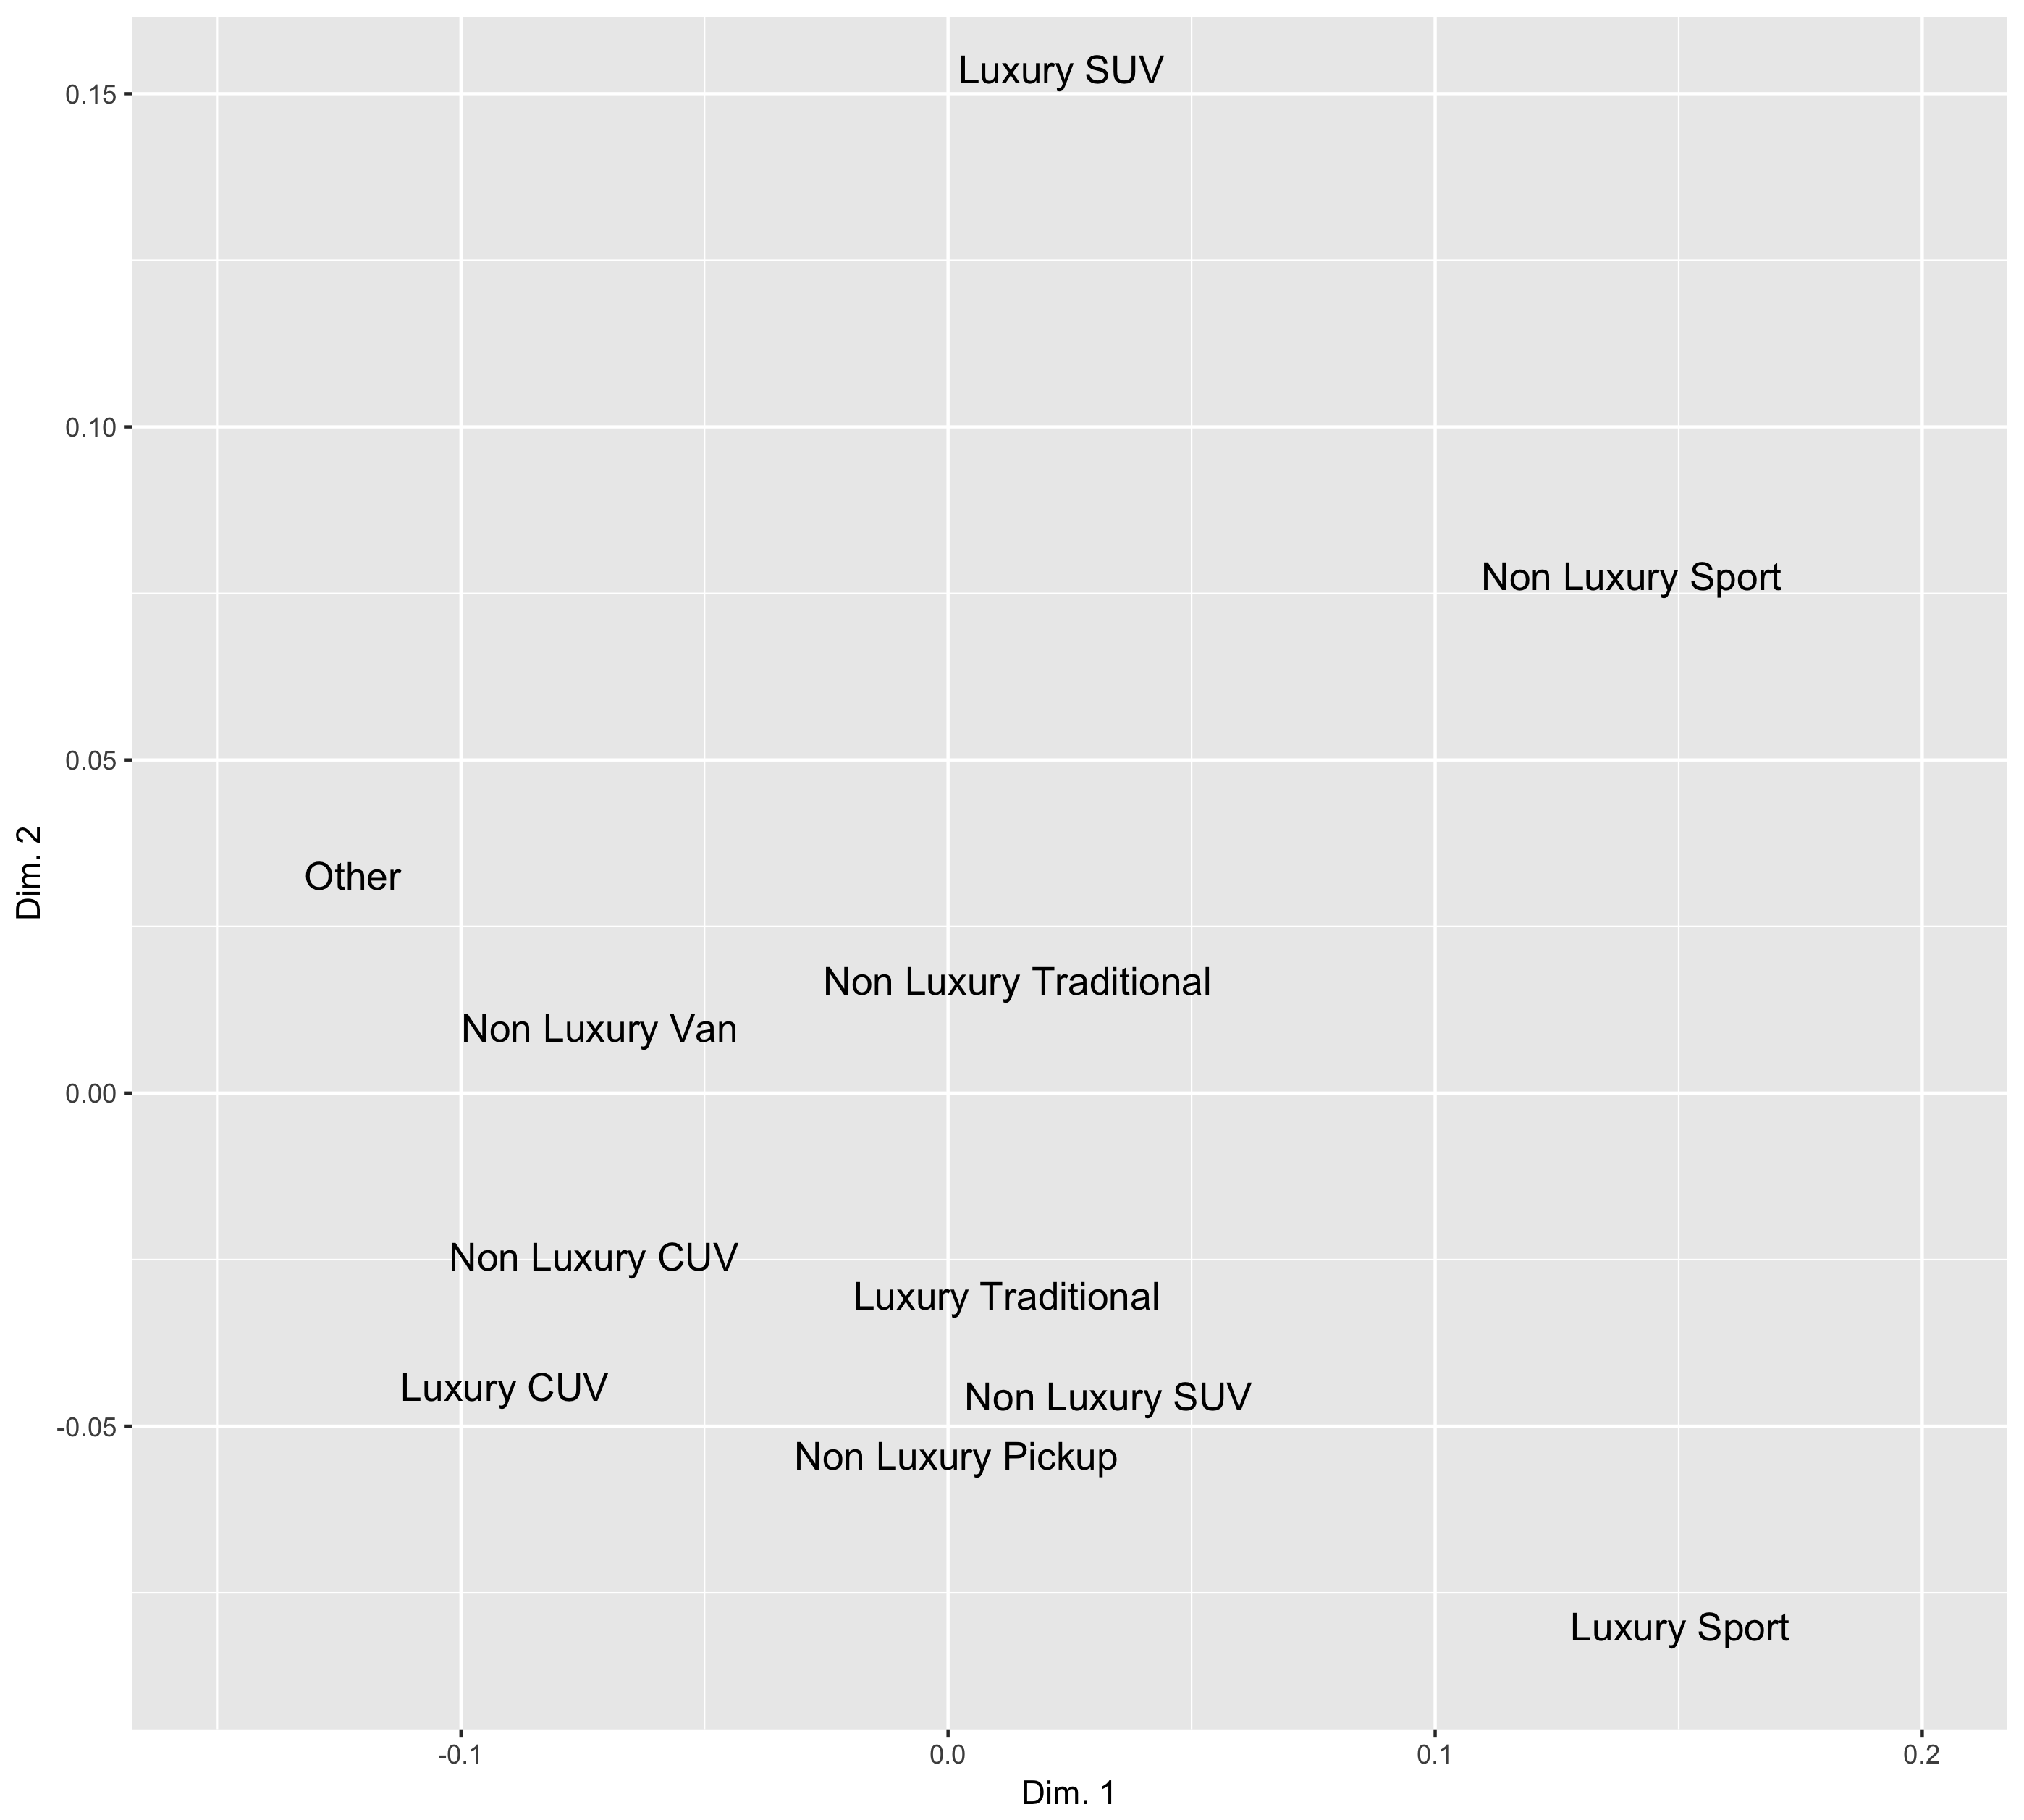
\includegraphics[width=1\linewidth]{VehicleTypeMDSPlot.png}
  \caption{Vehicle Type MDS}
  \label{fig:sub2}
\end{subfigure}
\caption{Multidimensional Scaling for Vehicle Manufacturer and Vehicle Type}
\label{fig:test}
\end{figure}

The plots don't indicate strong patterns of differentiation, but there are some noteworthy indicators. In particular, these results suggest that luxury sport/SUV drivers behave distinctively, as noted by the outlying values for the BMW/Land Rover\footnote{Note that this analysis considers all Jaguar models to manufactured by Land Rover} in figure (a), and for Luxury SUV and Sport vehicles in figure (b).

To explore the relevance of automaker in the context of actual prediction, we draw on various classifiers, in order to assess (a) is there any relationship between the make of a car and the likelihood of a multi-fatality incident, and (b) how important is this relationship, when compared alongside other important indicators of driver behavior. To more easily address part (a), we employ logistic regression for ease of interpretation. For the latter point, we pursue SVM and AdaBoost-based classification for their greater predictive power.\footnote{Note again that the data in this report are drawn solely from accidents involving at least one fatality. Therefore, classification of multi-fatality accidents are predicting the likelihood of such an outcome, \textit{given that a fatal accident has already occurred.}}

To explore this issue, we generated a binary 1-0 indicator for whether an incident involved more than 1 fatality, and tested the classification performance of a series of different models, the results of which are shown below. To overcome the class imbalance issue, we employ the resampling procedure employed by the SMOTE algorithm (for ``Synthetic Minority Over-sampling TEchnique"), developed by Chawla, et al. (2002). SMOTE uses a combination of over-sampling of the minority class and under-sampling of the majority to improve class balance.\\

The below table shows relative test error rates for classification using logistic regression, support vector machine, and adaptive boosting methods. \\

\begin{table}[H]
\centering
\begin{tabular}{cccc}
  \hline
 & Logistic Regression & Supp. Vec. Machine & AdaBoost \\ 
  \hline
Accuracy & 0.75 & 0.80 & 0.79 \\ 
   \hline
\end{tabular}
\caption{Test Set Prediction Accuracy} 
\end{table}

\textbf{Logistic Regression} \\
The table immediately below shows odds ratio coefficients for each of the automakers considered in this analysis, with BMW as the omitted reference category. A negative coefficient indicates a decreasing likelihood of a multi-fatality wreck, while a positive coefficient indicates the opposite. Some similarities to Figure 3 above jump out. Subarus and Land Rovers, for example, are here associated with relatively low probability of multi-fatality wrecks. However, these results suggest, contrary to what we might have assumed from Figure 3, that Volkswagens, Hondas, and Mazdas have the highest positive relationship with the probability of high fatality. Both analyses, however, point to a common conclusion that the typical concerned motorist or non-motorist should feel more secure around Subarus and luxury car brands, and less so around vehicles produced by the largest automakers (Ford, etc.). 

\begin{table}[H]
\centering
\begin{tabular}{cl}
  \hline
 Odds Ratio & Automaker \\ 
  \hline
  0.85 & Volkswagen \\ 
  0.70 & Honda \\ 
  0.62 & Mazda \\ 
  0.50 & Ford \\ 
  0.41 & Toyota \\ 
  0.39 & Volvo \\ 
  0.39 & FCA/Chrysler \\ 
  0.33 & GM \\ 
  0.27 & Hyundai-Kia \\ 
  0.21 & Mitsubishi \\ 
  0.10 & Daimler \\ 
  0.06 & Nissan \\ 
  -0.07 & Subaru \\ 
  -0.34 & Land Rover \\ 
   \hline
\end{tabular}
\caption{Automaker Odds Ratios for Predicting Multi-Fatality Accident (Relative to BMW)} 
\end{table}

The below table consists of estimates of odds ratios for the other predictors considered in the logistic regression, in order to indicate their relationships with the outcome when controlling for a vehicle's make. Their relevance is discussed in greater detail below. In brief, there are some fairly common sense results here, such as that not wearing any restraint, driving too fast, being distracted, and consuming drugs/alcohol are all habits positively associated with the probability that a fatal wreck led to multiple deaths. Some other more curious results emerge, as well. For example, a higher record of previous crashes, DWI convictions, and license suspensions/revocations is actually negatively correlated with the likelihood of high fatality.

\begin{table}[H]
\centering
\begin{tabular}{cl}
  \hline
 Odds Ratio & Variable \\ 
  \hline
  0.26 & Distracted \\ 
  1.40 & On Drugs \\ 
  0.73 & No Restraint \\ 
  0.85 & Hit-and-Run \\ 
  0.66 & Speeding \\ 
  -0.29 & Previous Recorded Crashes \\ 
  -0.33 & Previous DWI Convictions \\ 
  -0.04 & Prev. Rec. Suspensions/Revocations \\ 
   0.01 & Travel Speed \\ 
   0.66 & Drunk \\ 
   0.68 & Inclement Weather \\ 
   0.44 & Intersection \\ 
   -0.00 & Hour of Crash \\ 
   \hline
\end{tabular}
\caption{Predictor Odds Ratios} 
\end{table}

\textbf{SVM and AdaBoost}

For our concerned motorist or non-motorist, it is worth addressing the level of attention that should actually be paid to the make of a given car, relative to other factors such as intoxication or distracted driving. To investigate this issue, we reference the below output, which illustrates variable importance rankings for the SVM and AdaBoost classifiers. The models don't completely agree on relative variable importance, but there are some key patterns. For example, key for both models is the fact that the hour of crash is a dominant predictor of the likelihood a fatal accident resulted in multiple deaths. In addition, a driver's record, potential drug use, and driving speed are especially significant for predicting multi-fatality accidents. Interestingly, whether or not a driver was distracted (using a cellphone, for example), and whether the weather was clear or not, appear to be relatively less significant determinants of the likelihood that a fatal accident involved multiple deaths. Further assessment of this question would consider the affect of these less important predictors on non-fatal accidents, as well as fatal ones. Finally, this analysis suggests that, within the context of other fatality-relevant predictors, automaker (labeled as``Makers" in the plot) is relatively unimportant. Accounting for various driver behaviors captures much of the meaningful risk in multi-fatality wrecks. \\

\begin{figure}[H]
\centering
  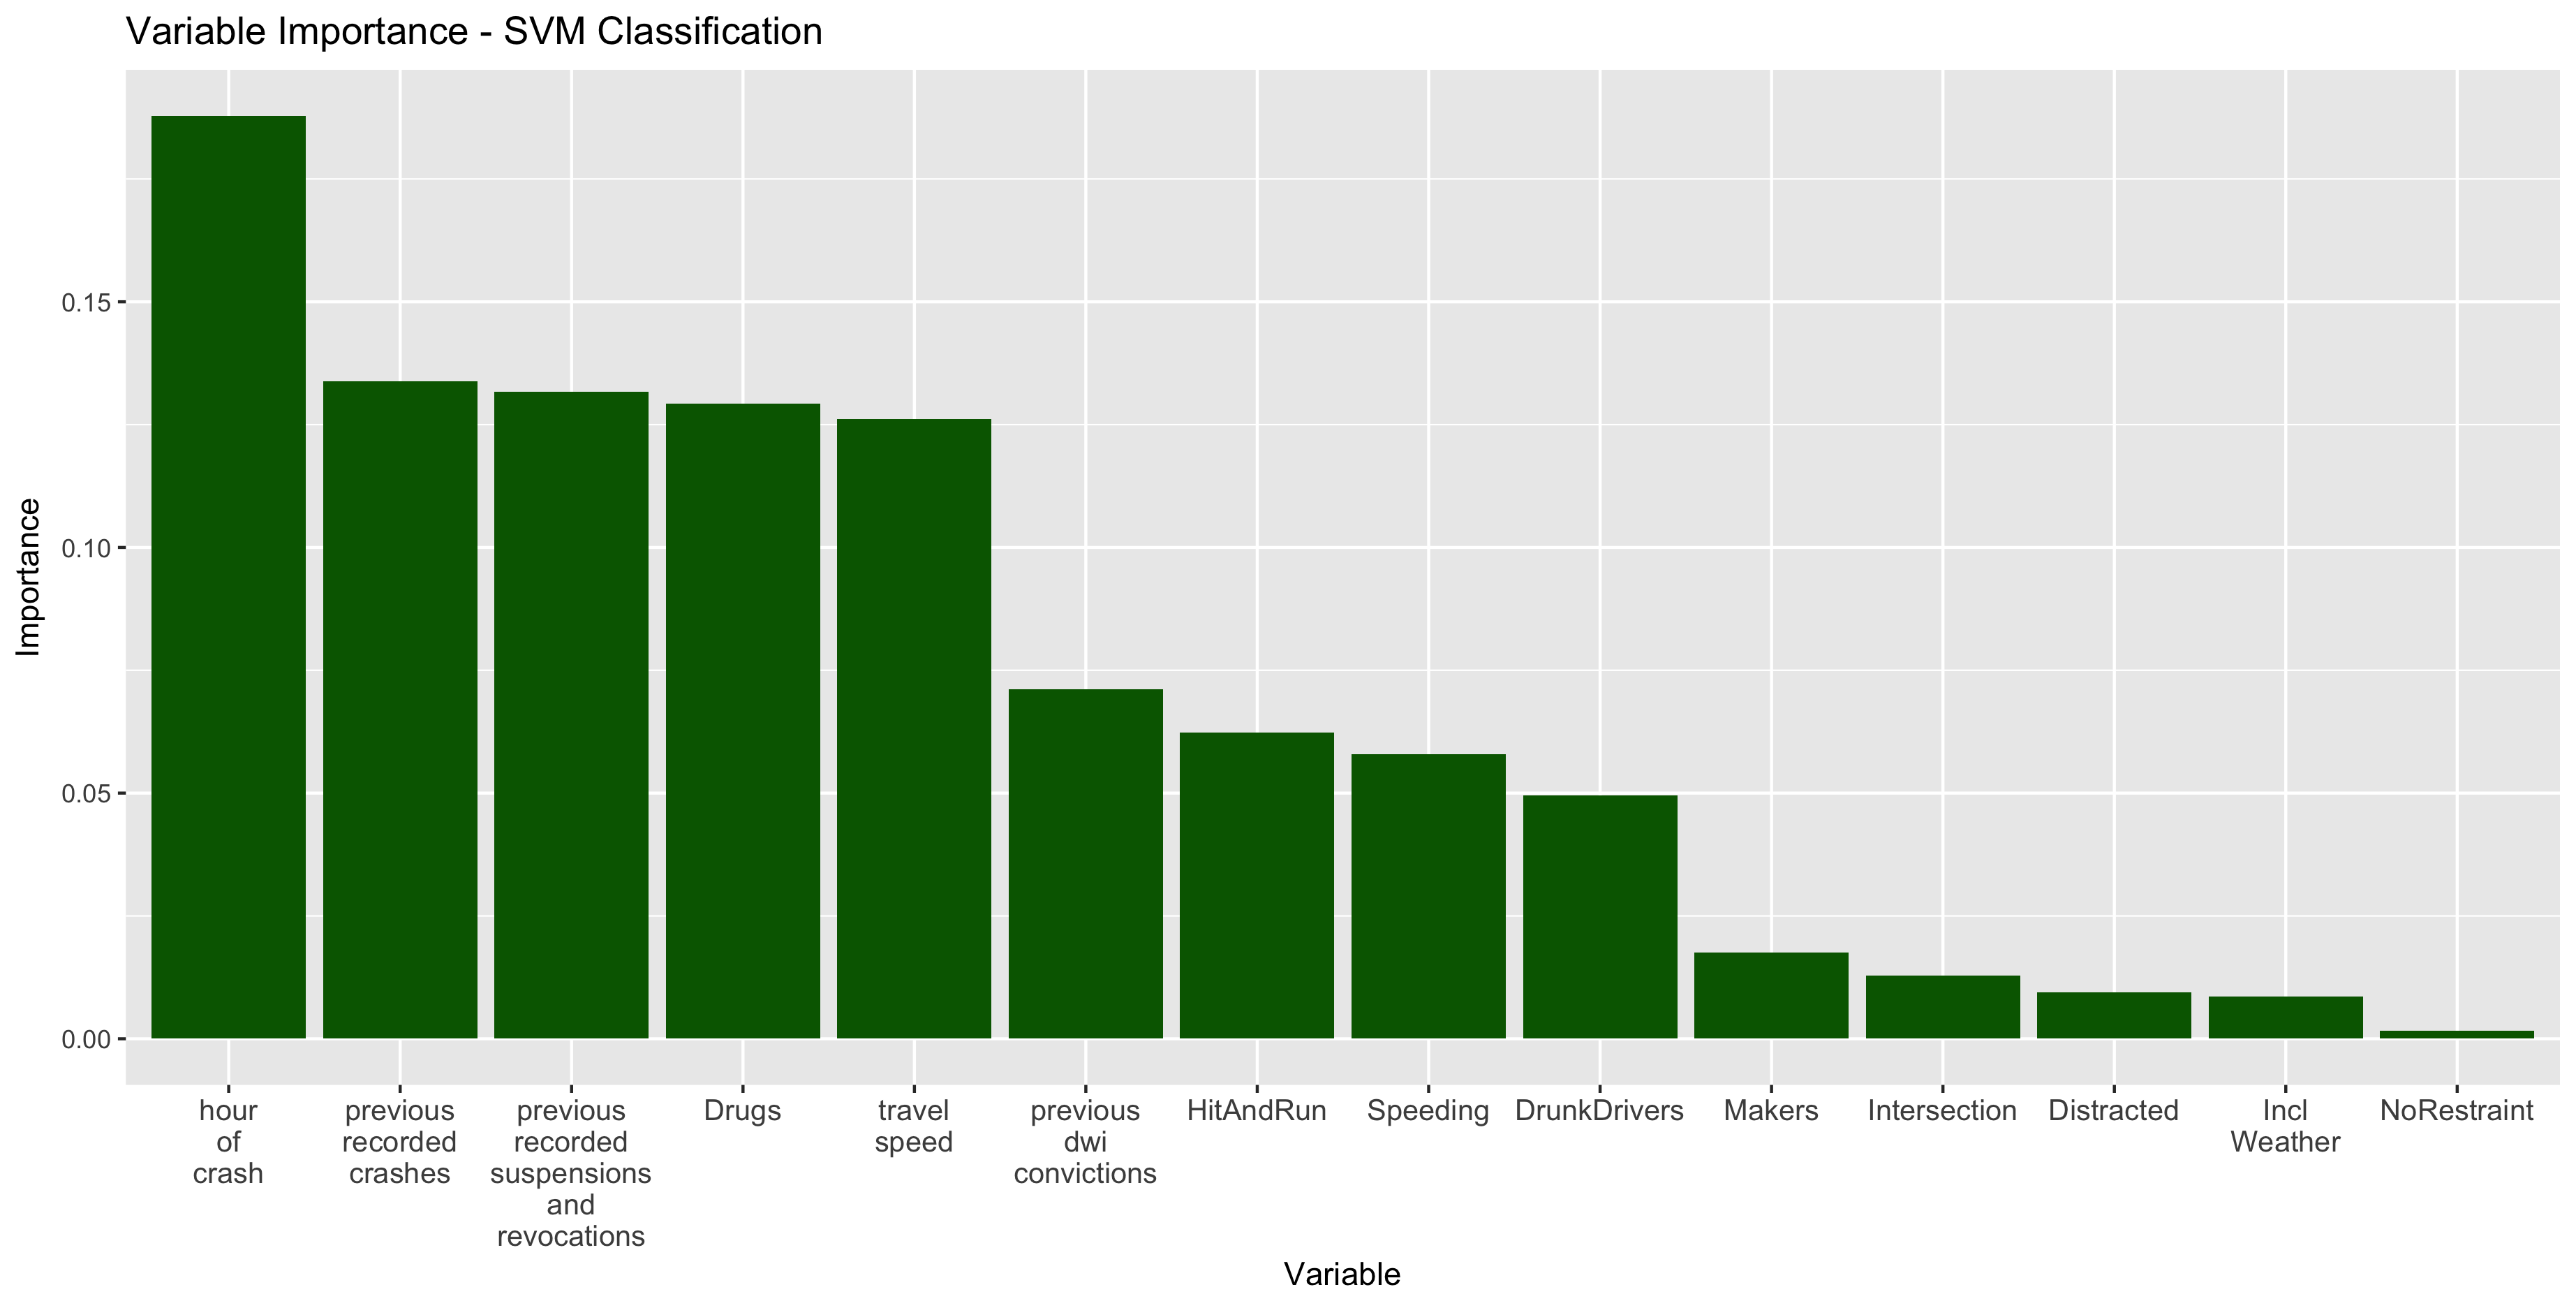
\includegraphics[width=15cm,height=8cm,keepaspectratio]{ImportancePlot_SVM.png}
\caption{Variable Importance - Support Vector Machine}
\end{figure}

\begin{figure}[H]
\centering
  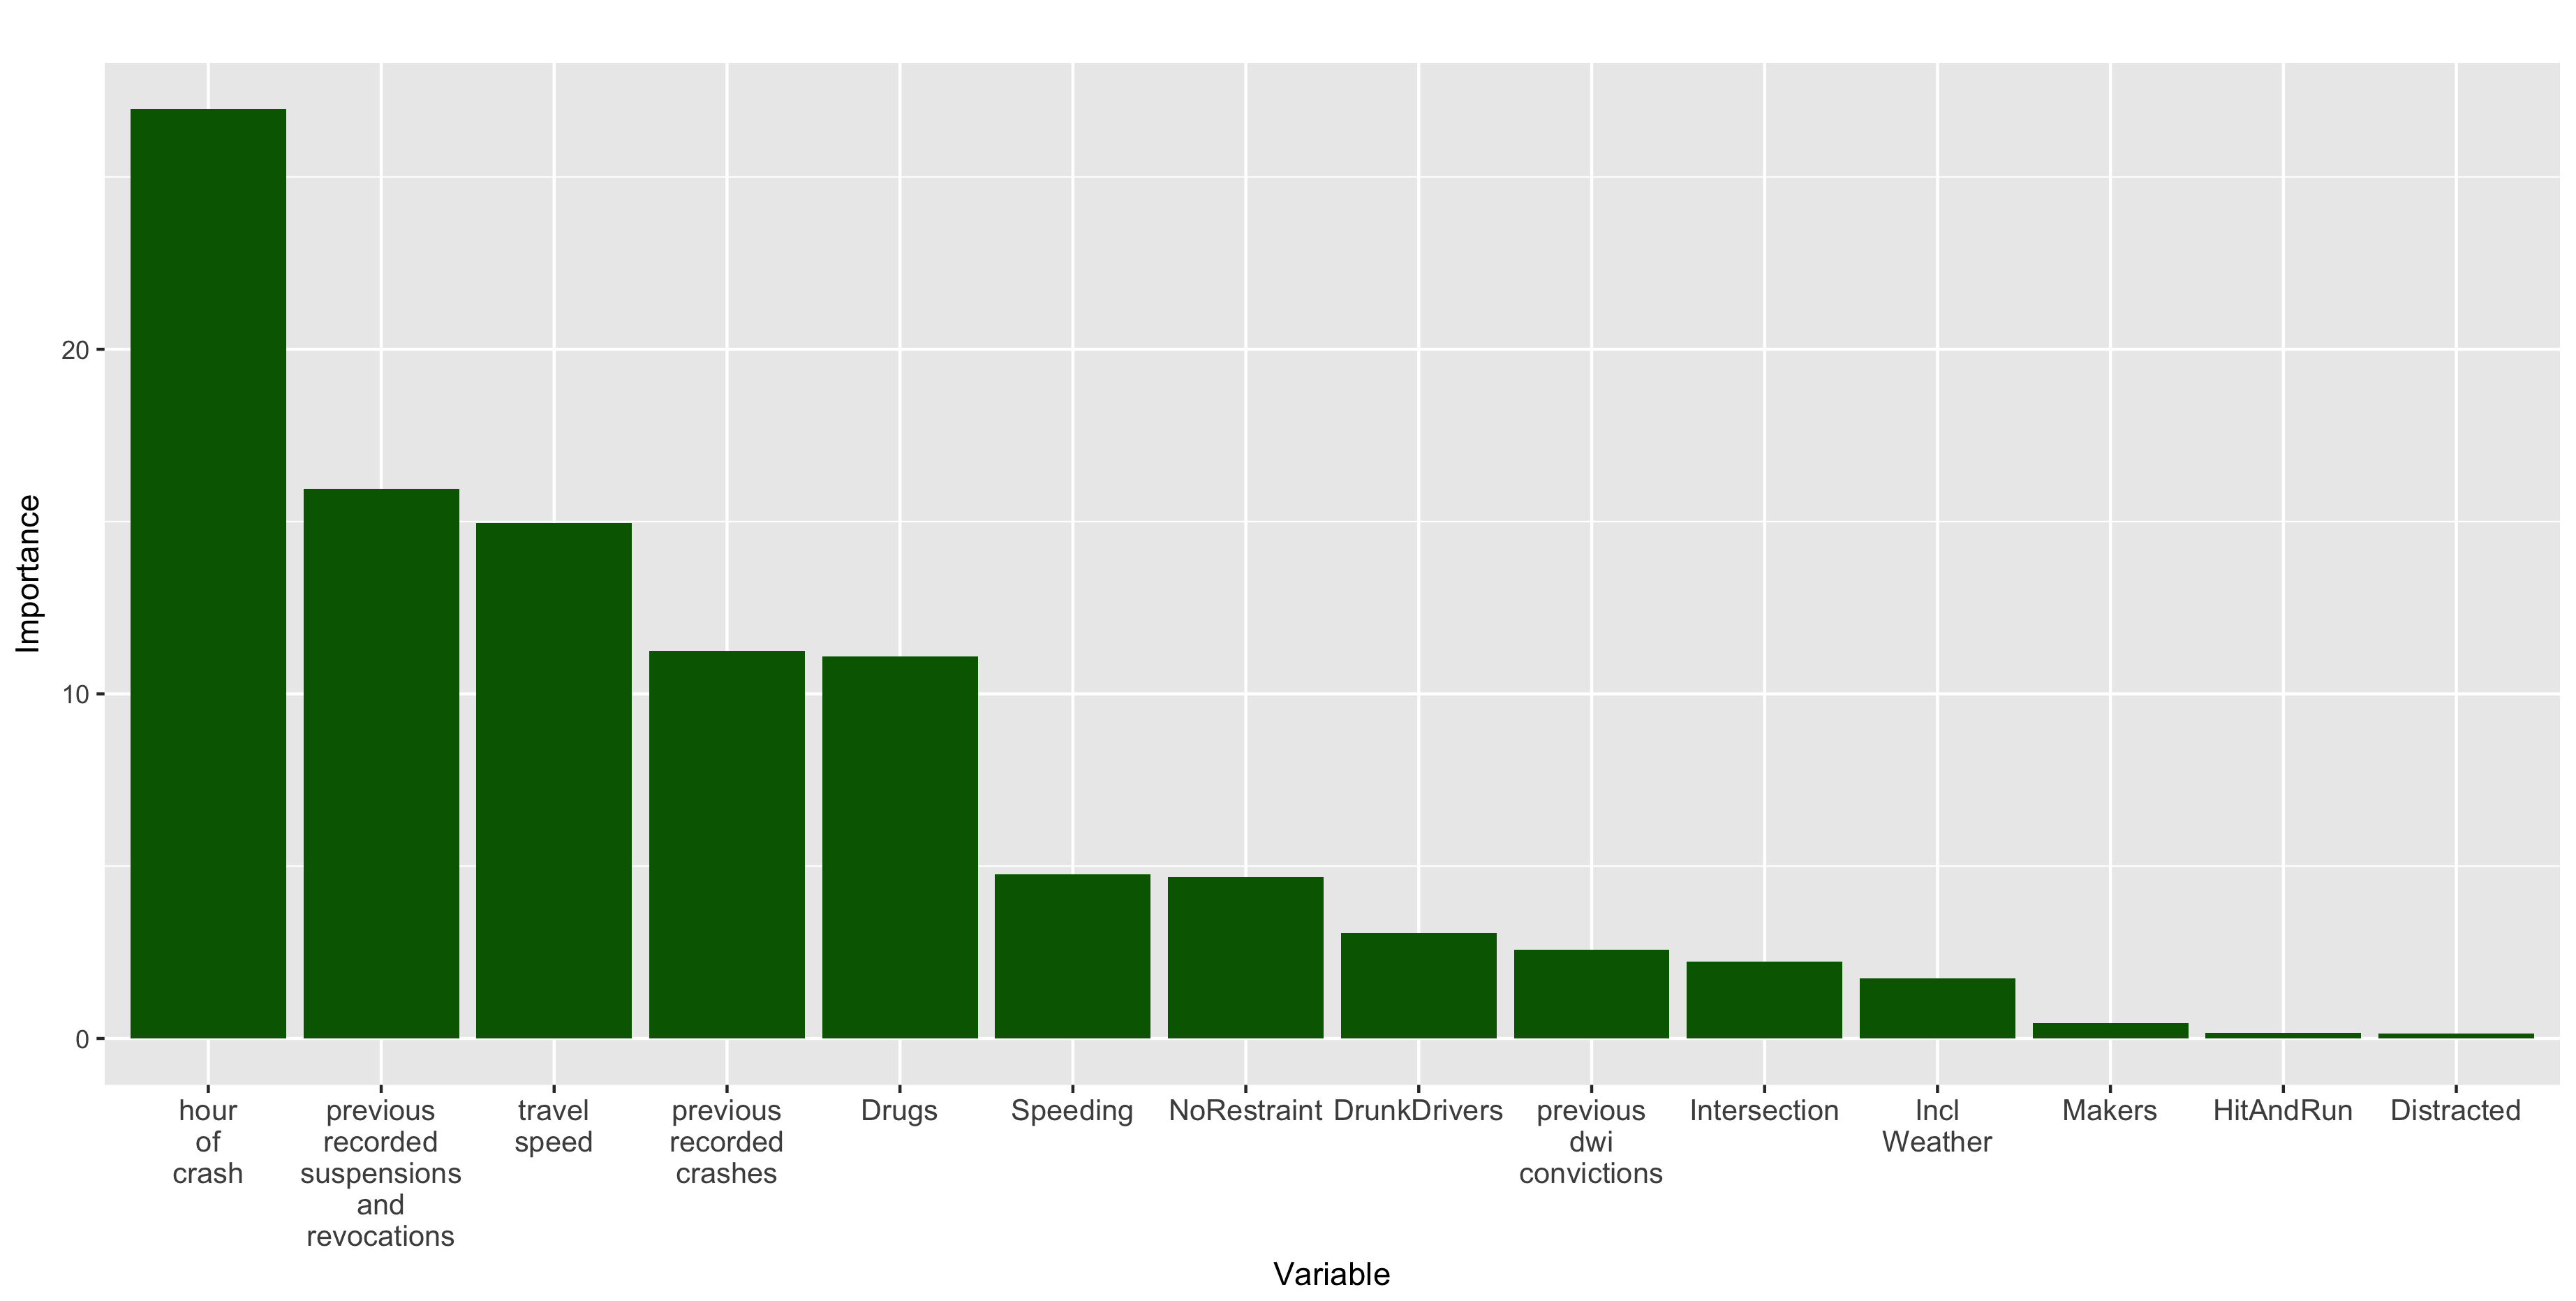
\includegraphics[width=15cm,height=8cm,keepaspectratio]{ImportancePlot_ADABoost.png}
\caption{Variable Importance - AdaBoost Algorithm}
\end{figure}

The below two sections explore in further detail the issues of driver impairment and hit-and-run incidents.

\section*{Driver Impairment}

An important predictor for high fatality accidents seems to be driver impairment. Impairment, as we are observing it, is a factor variable with 13 different possible values that focus on different types of impairment. On this new variable, we performed several different types of classifications methods to see whether impairment is an influential predictor.

\textbf{Logistic Regression}

The odds ratio of the logistic regression gives a relative measure of effect from the predictor variable to the response variable. Below is a table with the odds ratio given for each type of impairment in the impairment variable.  What is shown is that blind, deaf, and cane/crutches shows small/no effect on the response variable, but all of the other variable have a much larger effect on the response variable, with the impairment type of ``Other Impairment" having the largest odds ratio. What is interesting is influence of alcohol or drugs seems to have the smallest positive measure of effect, with subjects being in a wheelchair, being emotional, or begin blacked out having a larger measure of effect.

\begin{table}[ht]
\centering
\begin{tabular}{rlr}
  \hline
 & Impairment & Odds \\ 
  \hline
1 & Blind & 0.20 \\ 
  2 & Deaf & 0.19 \\ 
  3 & Emotional & 13.43 \\ 
  4 & Blackout & 13.89 \\ 
  5 & Impaired Due to Previous Injury & 14.73 \\ 
  6 & None/Apparently Normal & 14.76 \\ 
  7 & Not Reported & 14.16 \\ 
  8 & Wheelchair & 12.95 \\ 
  9 & Other Impairment & 15.69 \\ 
  10 & No Details & 0.18 \\ 
  11 & Influence of Alcohol or Drugs & 12.06 \\ 
  12 & Cane or Crutches & 0.05 \\ 
  13 & Unknown & 14.03 \\ 
   \hline
\end{tabular}
\caption{Predictor Odds Ratios}
\end{table}

The logistic regression we have generated shows a smaller error rate than the error rate given for the logistic regression of the car manufacturers. The error rate of the logistic regression is .088. This is directly, inversely related to the prediction accuracy given in the last section. A value of .088 error rate shows that the prediction we incorrect for that proportion of trials.

\textbf{GBM}

Another interesting type of classification is using generalized boosted models (GBM). GBM can be used to with several different distributions to show which variables have influence on the response variable. There are three different distributions that can be used with this response variable: Bernoulli, Huber, and AdaBoost. Bernoulli applies when there is a 0-1 outcome on the response, Huber applies a Huberized hinge loss function on the response, and AdaBoost applies an exponential loss function on the response. The following table provides the error rates associated with each distribution.

\begin{table}[H]
\centering
\begin{tabular}{cccc}
  \hline
 & Bernoulli & Huber & AdaBoost \\ 
  \hline
Error Rate & .121 & 0.0911 & 0.0804 \\ 
   \hline
\end{tabular}
\caption{Test Set Prediction Error Rate} 
\end{table}

What we can see from these error rates is that the normal Bernoulli distribution has the largest occurrence of errors within the test data, while the AdaBoost distribution has the smallest occurrence of errors.

\textbf{Decision Tree}

Decision trees can also be useful in predicting whether a specific accident is a high fatality accident or not. We created a decision tree with the same predictors as before and evaluated the error rate from the tree. The error rate we received is .0934. When comparing this to the logistic regression and the boosted regressions, we can see that the decision tree produces higher error rates than all of the regressions other than the Bernoulli GBM regression error rate, which is the simplest of all of the models. Most likely due to the large number of predictors and the large number of factors within each predictor, the decision tree has a larger error rate than other forms of classification.

\section*{Hit-and-Run}
In this section we will discuss hit-and-run behavior as it brings more risk of fatalities during traffic accidents. According to a 2014 NHTSA traffic safety factsheet (see references), nearly one in five pedestrians killed in traffic crashes were involved in hit-and-runs. As such, it is an especially relevant factor to consider for non-motorists. To assess relationships of various predictors with hit-and-runs, we run a logistic regression, with a binary 0-1 indicator for hit-and-run as the outcome, and representative driver behavior and natural features such as spending, past driving history and time of the accident are used as independent variables. We employ logistic regression primarily because the focus is on inference rather than prediction. where hit-and-run as dependent variables . With some model selection, we get the following regression result.

Hit-and-runs are a relatively rare event. Thus, we again employed resampling techniques to adjust for class imbalance, oversampling the minority class (hit-and-run = 1) and undersampling the majority class (hit-and-run = 0). In comparing resampled data (results shown below) with the original imbalanced data set, there did not appear to be significant difference in coefficient estimates.

\begin{table}[!htbp] \centering 
	\label{} 
	\begin{tabular}{@{\extracolsep{5pt}}lc} 
		\\[-1.8ex]\hline 
		\hline \\[-1.8ex] 
		& \multicolumn{1}{c}{\textit{Dependent variable:}} \\ 
		\cline{2-2} 
		\\[-1.8ex] & Hit-and-Run \\ 
		\hline \\[-1.8ex] 
		Distracted & 0.216$^{***}$ (0.025) \\ 
		Drugs & 0.307$^{***}$ (0.048) \\ 
		MultiFatality & $-$1.059$^{***}$ (0.050) \\ 
		Speeding & 1.018$^{***}$ (0.029) \\ 
		Previous Recorded Crashes & 0.004 (0.020) \\ 
		Previous DWI Convictions & 0.777$^{***}$ (0.040) \\ 
		Previous Recorded Suspensions and Revocations & 0.158$^{***}$ (0.007) \\ 
		DrunkDrivers & 0.110$^{***}$ (0.028) \\ 
		Daytime & $-$0.816$^{***}$ (0.032) \\ 
		Evening & 0.153$^{***}$ (0.031) \\ 
		Constant & $-$1.270$^{***}$ (0.030) \\  
		\hline \\[-1.8ex] 
		\textit{Note:} Standard error is in bracket & \multicolumn{1}{r}{$^{*}$p$<$0.1; $^{**}$p$<$0.05; $^{***}$p$<$0.01} \\ 
	\end{tabular} 
	\caption{Predictors of Fatal Accidents Involving Hit-and-Runs}
\end{table} 

The results above suggest that speeding, previous DWI convictions and drug use are positively correlated with hit-and-runs. There is also a significant reduction in probability of hit-and-runs during the daytime (7am to 6pm) compared with the night and evening.

It is interesting to note that the indicator of multiple fatalities has a significantly negative coefficient. This may be due to the fact that hit-and-runs are commonly involved in collisions with pedestrians, which may be less likely to result in multiple fatalities when compared with multi-vehicle collisions. In addition, a multiple-fatality crash might mean a severe crash that is more likely to total a given car, preventing the driver from fleeing the crash.


\section*{Environmental Factors}
The concerned motorist may also worry about the weather, in addition to the issues we have considered throughout this report. A proper analysis of environmental factors is both beyond the scope of this analysis, and requires incorporating a richer set of weather data than the handful of indicators available in the FARS system. A quick initial check of the relevance of environmental conditions doesn't return many relevant results. The plot below shows data from Cook County, Illinois, chosen for its high number of traffic fatalities and variable weather\footnote{Especially when compared to Dallas, Phoenix, and LA County}. The vast majority of fatal collisions occur in clear weather, which is due in large part no doubt to the fact that it is simply clear much more often in Chicago than it is rainy or snowy! 

\begin{figure}[H]
\centering
  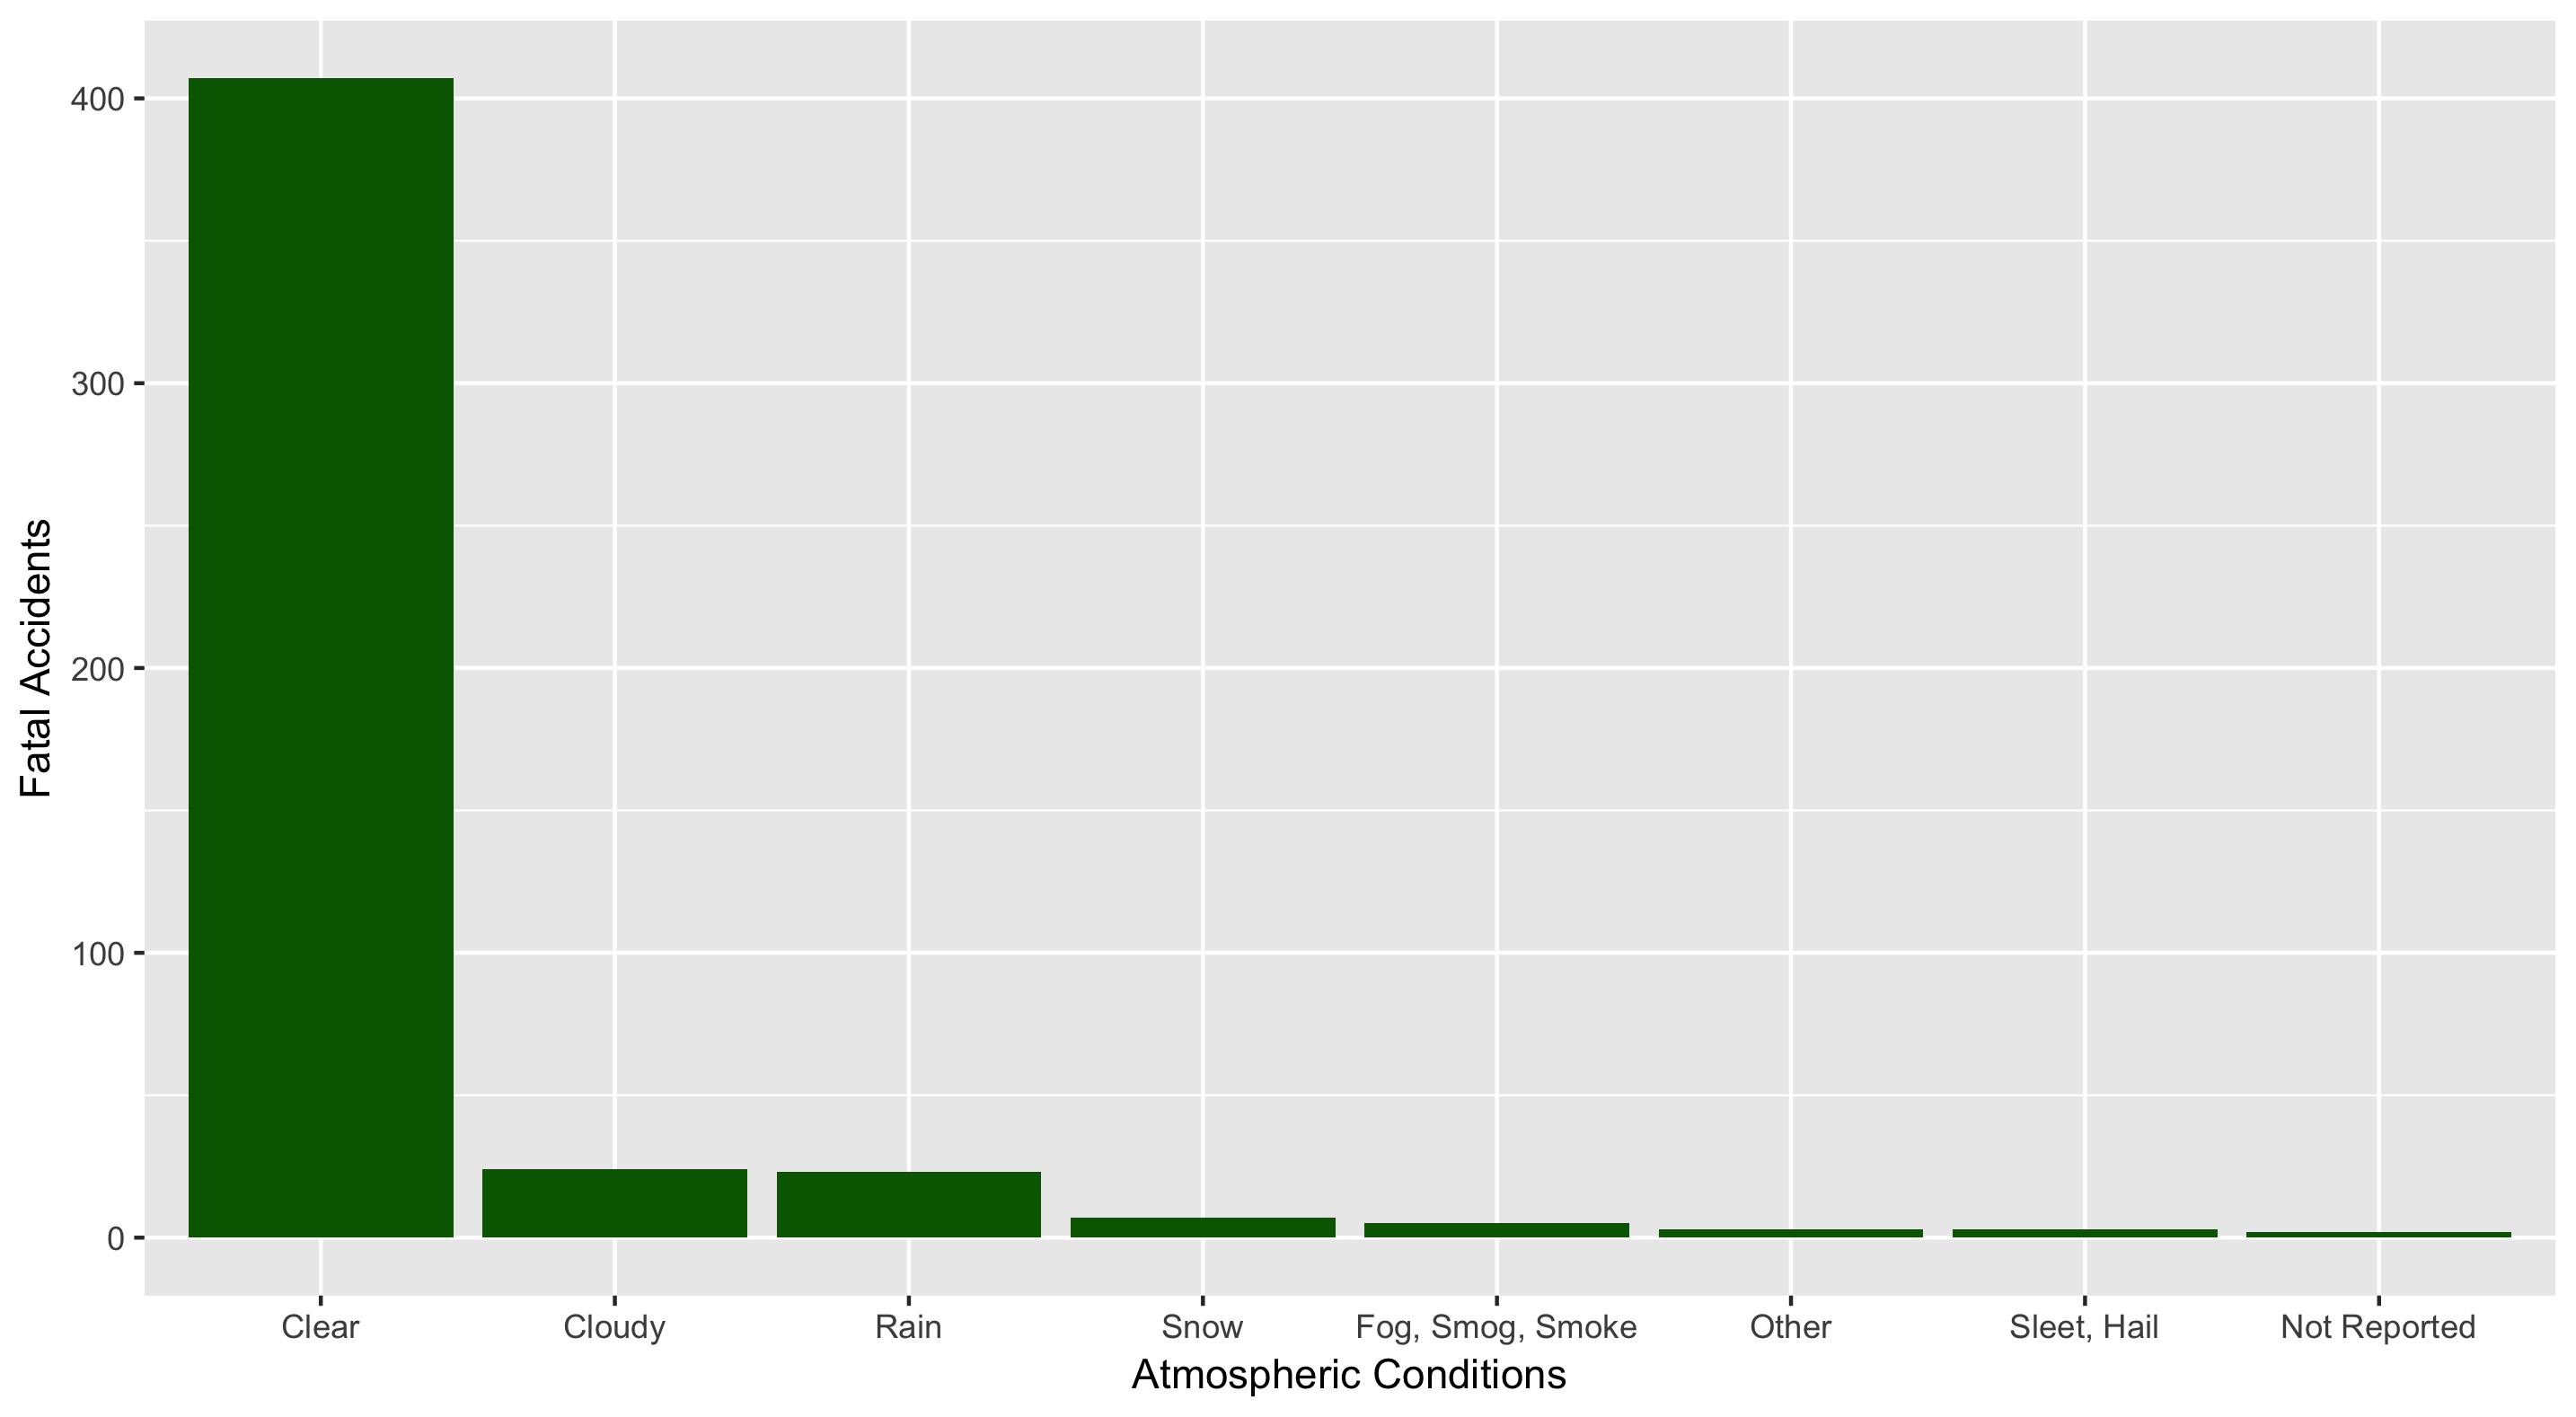
\includegraphics[width=15cm,height=8cm,keepaspectratio]{Environmental.png}
\caption{Fatal Accidents in Cook County, by Atmospheric Condition}
\end{figure}


\section*{Conclusion}

Many of the issues considered in this analysis will likely already have been considered by the well-prepared motorist or non-motorist. However, they bear repeating, alongside some recommendations that may surprise the average reader. In particular:

Where to Drive: Fatality rates seem to be the highest on highways of less densely packed states. More fatal accidents do occur in higher population states, but population density seems to indicate that more accidents occur per capita for larger states in area. So, it is optimal to drive on local roads with lower populations in high densities, if at all possible.

When to Drive: Fatality rates are consistently highest between midnight and 5AM throughout much of the country. The hour of a crash is also a key determinant of the probability that an accident results in multiple fatalities.

Which Cars to Avoid: Steer clear of the largest automakers, and rest easier among Subarus, BMWs, Jaguars, and Range Rovers.

Which Drivers to Avoid: Drivers on drugs or alcohol, distracted drivers, drivers not wearing seatbelts, and drivers traveling at high speeds.


\section*{References}
\begin{hangparas}{1.27cm}{1}
Batterman, Stuart, Richard Cook, and Thomas Justin. ``Temporal variation of traffic on highways and the development of accurate temporal allocation factors for air pollution analyses." \textit{Atmos Environ}. Apr. 2015.

Chawla, Nitesh, Kevin Bowyer, Lawrence Hall, and W. Philip Kegelmeyer. ``SMOTE: Synthetic Minority Over-sampling Technique." \textit{Journal of Artificial Intelligence Research}. 2002.

Choi, Eun-Ha. ``Crash Factors in Intersection-Related Crashes: An On-Scene Perspective." \textit{U.S. Department of Transportation - National Highway Traffic Safety Administration}. Sept. 2010.

Gravano, Luis and John Paparrizos. ``k-Shape: Efficient and Accurate Clustering of Time Series." \textit{SIGMOD}. June 2015.

Zador, P.L, S.A. Krawchuk, and R.B. Voas. ``Relative Risk of Fatal Crash Involvement by BAC, Age, and Gender." \textit{U.S. Department of Transportation - National Highway Traffic Safety Administration}. Apr. 2000.

``National Motor Vehicle Crash Causation Survey: Report to Congress." \textit{U.S. Department of Transportation - National Highway Traffic Safety Administration}. July 2008.

``2014 Traffic Safety Factsheet Pedestrians." \textit{U.S. Department of Transportation - National Highway Traffic Safety Administration}. May 2016.

\end{hangparas}




\end{document}  
